\citet{2022A&A...664A..31C} Laia's paper that used the first version of the code.

In this chapter, I summarize the works undertaken in this thesis and reconnect it to the broader literature with proposing more avenues for investigation. 

\section{Summary}
    In Chapter 1, I outlined the importance of stellar streams from globular clusters, highlighting both their intrinsic scientific interest and their role as probes for a wide range of astrophysical questions. These include the chemical enrichment of the Universe, the assembly history of the Milky Way, pathways of black hole formation, and constraints on the global and local properties of the Galactic gravitational field—particularly in relation to the detection of dark matter.

    In Chapter 2, I presented the exact equations of motion used to model the formation of stellar streams from globular clusters, formulated as a restricted three-body problem. I then explained how these equations can be interpreted to describe the escape of stars through the Lagrange points under tidal forces, followed by their evolution via phase mixing to form the streams. I summarized the literature on the mechanisms by which perturbations can create gaps. I also discussed the limitations of our models: specifically, that without $N$-body simulations or analytical prescriptions for internal cluster dynamics, certain questions cannot be addressed.

    In Chapter 3, I introduced my simulation code, \texttt{tstrippy}, describing its numerical solution of the equations of motion, its performance in terms of accuracy and computation time, and a comparison of two numerical schemes. I explained how the code is written in Fortran and interfaced with Python via \texttt{f2py}, and provided a minimal, {\tiny non}-working example illustrating the workflow from the user's perspective.

    In Chapter 4, I presented \citet{2023A&A...673A..44F}, in which we simulated the expected tidal debris from the entire globular cluster catalogue. These simulations have been made publicly available and are now used by the community, including in searches for additional tidal debris beyond some of the clusters in our sample \citep{2025arXiv250705590K,2025ApJ...988...39W}.
    
    In Chapter 5, I present \citet{2025A&A...699A.289F}, where we investigated how the Palomar~5 stellar stream responds to the granularity of the Milky Way's gravitational field—specifically, the presence of other globular clusters. We showed that the internal dynamics of globular clusters can strongly influence the morphology of their stellar streams. In particular, gap formation from the fly-by of a massive perturber requires very specific stream conditions: regions close to the progenitor, where the morphology is still dominated by epicyclic overdensities, are unfavorable for gap formation, as different stellar packets respond differently to the perturbation and subsequently drift out of phase. This is a new contribution, as previous studies primarily considered the effects of random motions, such as velocity dispersion.

\section{Prospectives}
    I think the good thing here is that we really focus on Milky Way streams and globular clusters. Idealized toy models and set ups are good for investigating new ideas and various types of theoretical phenomena \dots However, \dots by focusing on the Milky Way, we can truly \dots know how much of these we can expect to see, with what significance, and always tie back around to the observations \dots

    The ubiquity and sensitivity of stellar streams really do make them amazing for inferring properties of various distributions. There are thus various avenues of investigation that can be taken on next. Some phenomena still needs to be explored with numerical forward modeling. Either for understanding physical mecanisms, or for obtaining predictions on how often something should be observed. On the otherhand, where the phenomena is well understood we can turn to observations to begin actually perform the inference. 

    \subsection{Dark Matter}
        The question of inferring the presence of dark matter on lower-mass scales than from the extra-galactic context excites us. We aim to perform a similar study to Chapter~5, but in addition to only using the populating og galactic globular clusters, we would like to use a $\Lambda$CDM motivated population of dark matter subhalos (Boldrini et al. In prep). See Fig.~\ref{fig:mollweide-density-with-haloes.png} in which a population of dark matter sub-haloes from a cosmological simulation in a Milky Way analog is displayed. \citet{2024arXiv241213144A} recently performed a similar work for just the GD-1 stream. They found, that the GD-1 stream in the last few billion years has on average, one gap from the passage of a dark matter sub-halo. \citet{2025arXiv250207781L} used the average of $1$ gap per stream to discuss the observability about 50 known Milky Way streams. 

        \begin{figure}
            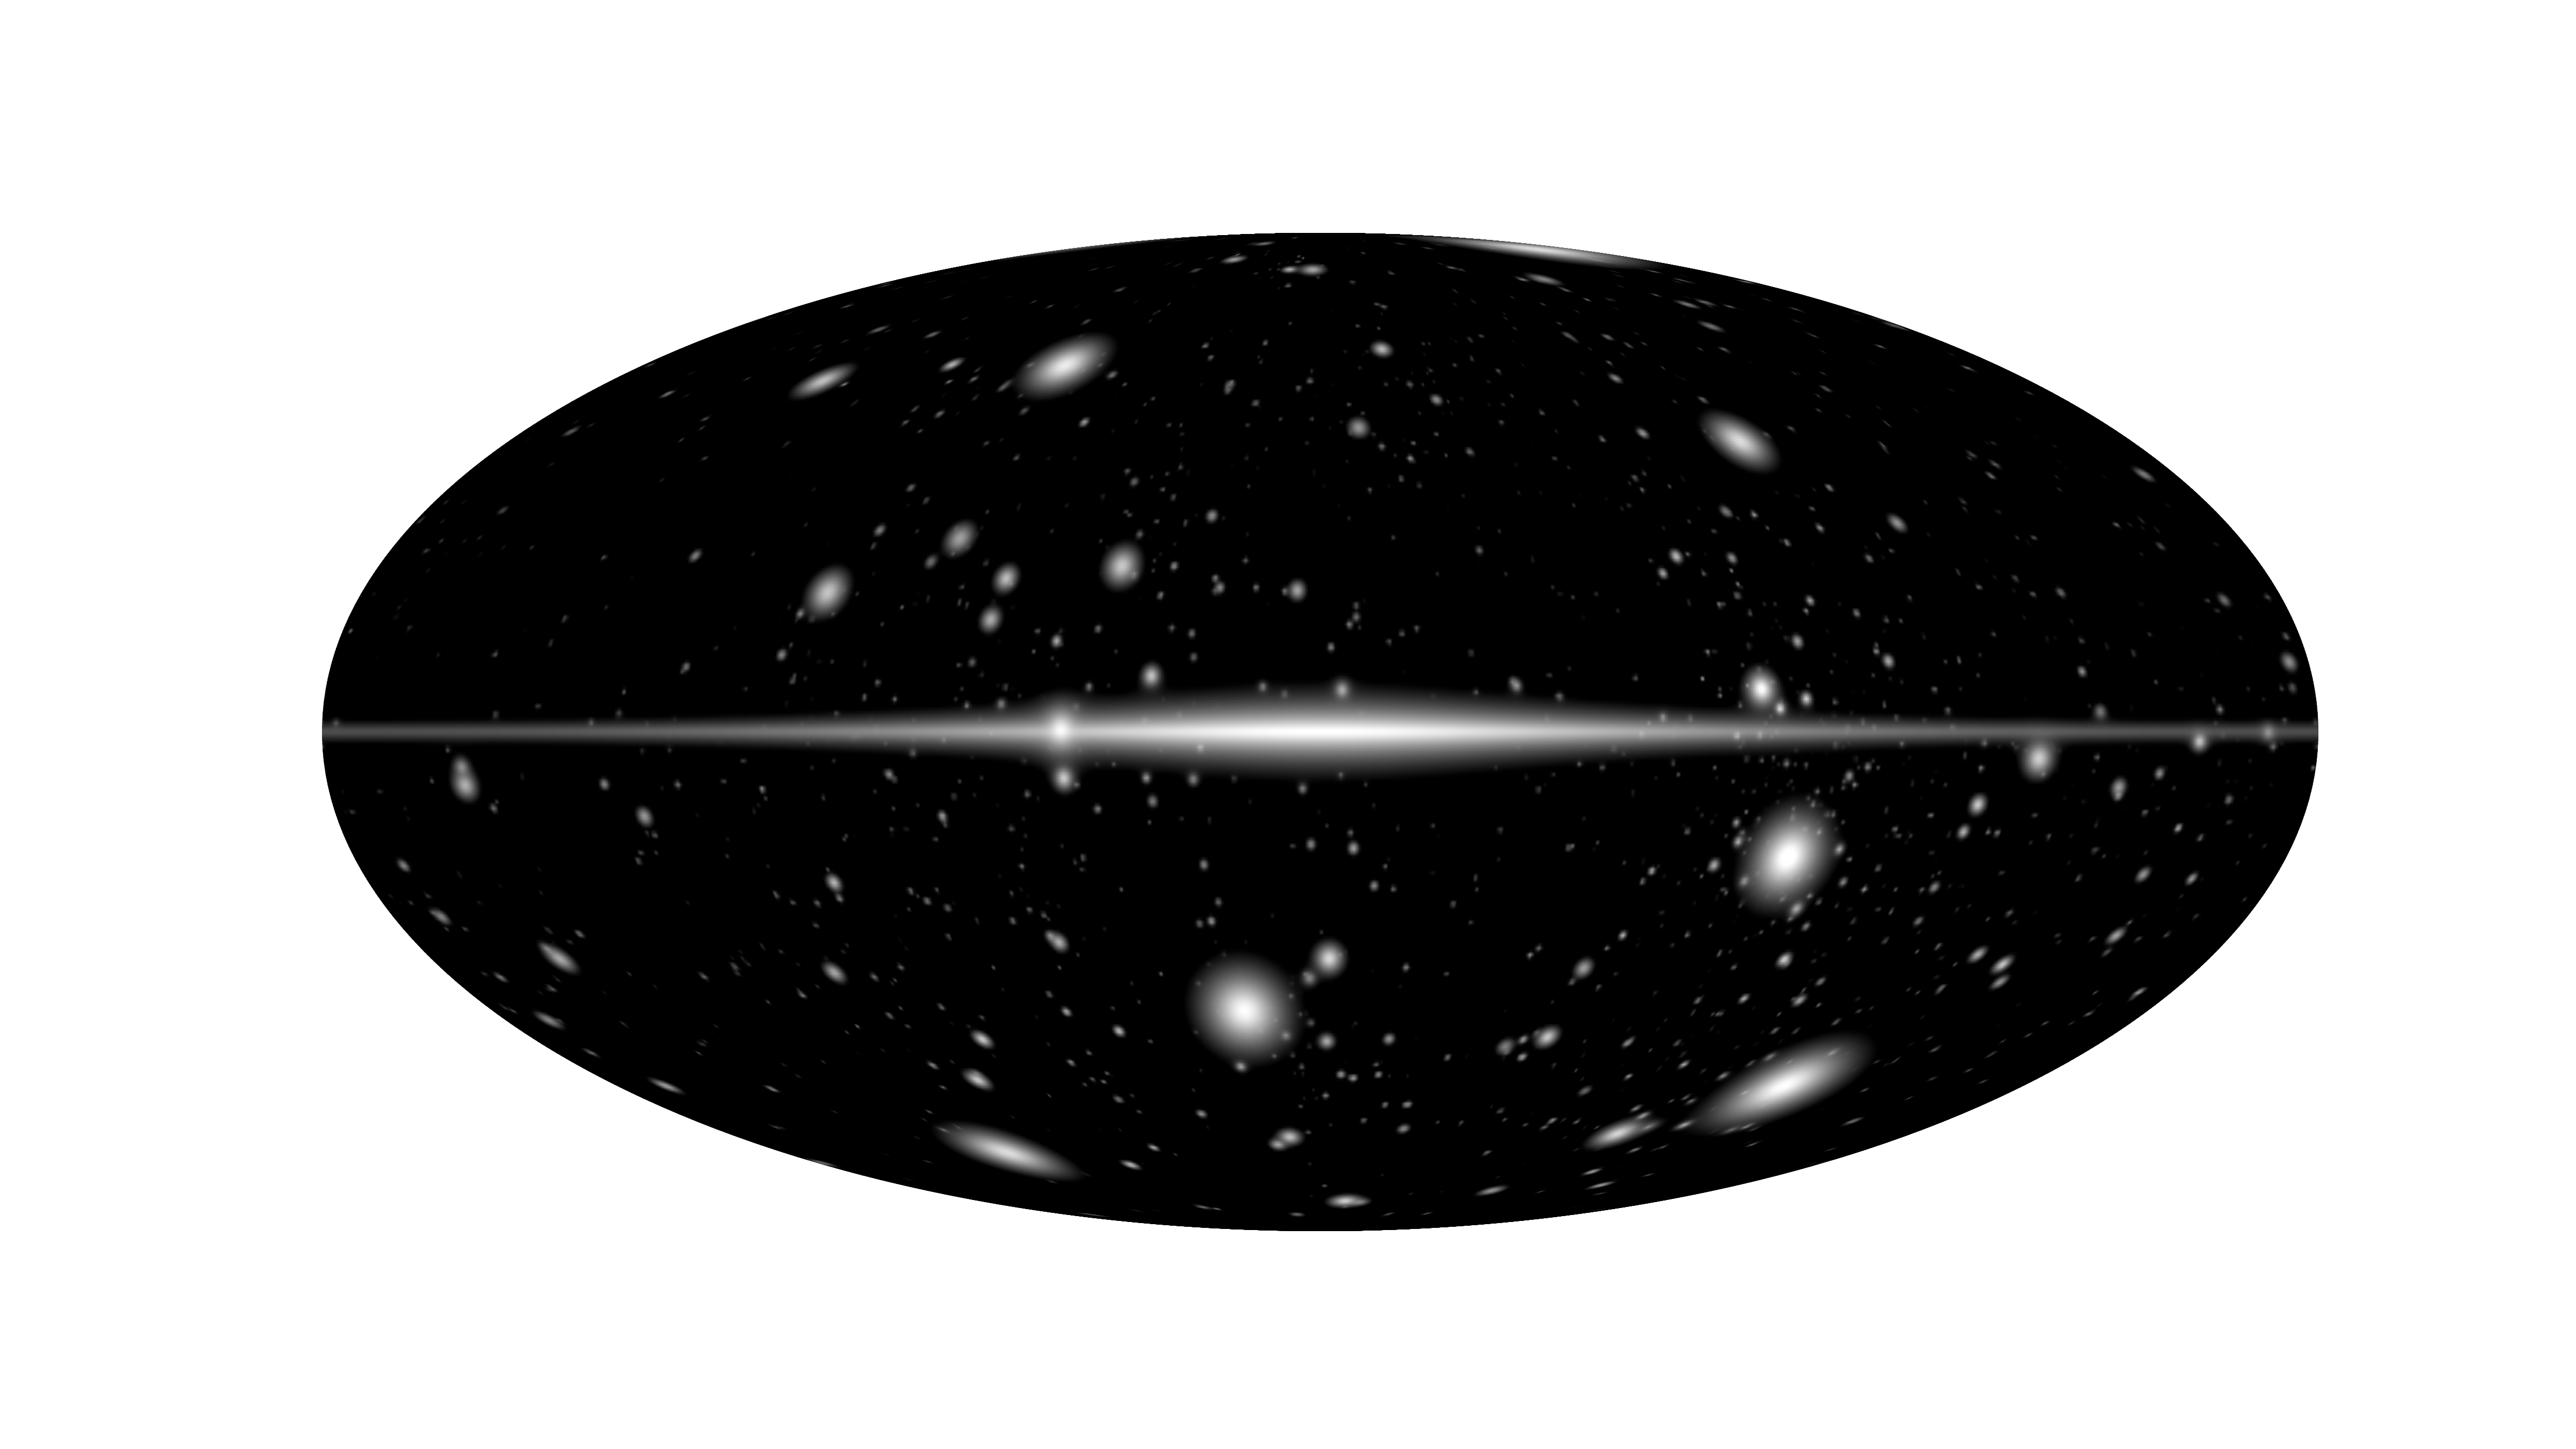
\includegraphics[width=\linewidth]{images/mollweide-density-with-haloes.png}
            \caption[Plausible $\Lambda$CDM Dark matter subhalo population as seen from the Sun]{Plausible $\Lambda$CDM Dark matter subhalo population as seen from the Sun. The subhaloes are modelled as Plummer sphere's and their light was integrated over the line of sight from the sun. Their ``luminosity'' was scaled as to the total halo's total mass. They are also overlain the integrated surface light density profile of Milky Way's stellar disk, as modeled with a Miyamoto-Nagai that models the Milky Way potential.}
            \label{fig:mollweide-density-with-haloes.png}
        \end{figure}

        There also exists more modeling to understand the phenomenon of gap formation in the Milky Way stellar streams. Yes, we want to do some theoretical predictions to know how many we should expect. However, it must be in a more realisitic Milky Way with other known time-dependent and non axis-symmetric features. Until now, studies have only considered subhaloes impacting streams in isolation \citep{2013ApJ...775...90C,2015MNRAS.450.1136E,2016MNRAS.463..102E,2016MNRAS.457.3817S,2024arXiv241213144A,2025arXiv250207781L}. Or just the effects of the galactic bar on individual streams in isolation \citep{2016MNRAS.460..497H,2016ApJ...824..104P,2017NatAs...1..633P,2023A&A...678A.180T}. However, it is known that perturbations of stream from ordinary matter gap explain gap signals that some attribute to the passage of dark matter halos \citep{2020ApJ...891..161I}. In order to properly set up the inference problem, the false positive rate must be known and calibrated. 

        Then, overall, fully inverting the problem is an example problem of bayesian hierarchical models \citep{2020sdmm.book.....I}. Interestingly, each gap detection is under-determined \citep{2015MNRAS.450.1136E}. Even in the absence of uncertainties, the presence of a gap cannot uniquiely and simultaneously determine the perturber mass, perturber size, time of impact, and relative velocity \citep{2015MNRAS.450.1136E}. However, with enough gaps and posterior distributions of each encounter, we can eventual build a statistic on the types of DM sub-halos.  

        This problem is tricky tricky. To solve it we need to understand other important physical processes that can erase signatures or contribute to false positives and in what quantity, and build a hierarchical model to complete the inference--let alone to apply this to the Milky Way have very high data quality. Quality that may be available with LSST and the final Gaia data releases.

        However, as highlighted in Chapter~5, the coherence within the stream is important for gap persistence and we must make sure they are modeled correctly or else we may have too many gaps. Of course, full $N$-body simulations maybe tempting to properly capture the internal dynamics of the cluster in order to propely map them to the streams. As discussed in \citet{2018ComAC...5....2V,2023LRCA....9....3S} there are many N body modeling techniques and the field is an active area of research. It is often at the avant-garde of hard-ware soft-ware synergy to create the fastest codes with the highest accuracy. For example, GRAPE, was hardware specifically used for this problem and was used until replaced by GPU \citep{2012MNRAS.424..545N,2015MNRAS.450.4070W}. Despite the advancements in both fields, they remain too expensive for the statistics that we require. Indeed, in order to properly theoretically calibrate our expectations for inferring dark matter sbhalos. we may need to run over a parameter space including different various models for the Galaxy's gravitational field, internal dynamics of the cluster, orbial initial conditions, dark matter-subhalo populations, various streams, etc. We can design an experiment in which we must compute tens of thousands of streams. 


        \begin{enumerate}
            \item this is where I will highlight some particle spray codes with semi-analytical methods. Perhaps I can switch to this or be more smart, like how Adams only simulated the orbits at first, but then simulated the streams once there was a close encounter. 
        \end{enumerate}


        \citet{2012MNRAS.420.2700K} created the ``streak-line'' method, which in essence approximates streams as having the same orbital parameters as the progenitor. \citet{2014ApJ...795...94B} continued this and used it to quickly generate streams in a monte-carlo code to find the best halo parameters to reproduced observed streams to recover a galaxy's mass. They generate orbits on the fly giving the star particles the same parameters as the progenitor but offset. 

        The ``streak-line'' method is limited and ignores the dispersion in orbital parameters of the escaped stars. \citet{2011MNRAS.413.1852E} presented streams in action-angle variables. As stated by \citet{2015MNRAS.452..301F}, this is the most elegant description of stellar streams. Each stream star has an offset from the progenitor's hamiltonian which can be expressed with a second order taylor expansion. 

        \citet{2015MNRAS.452..301F} prescriptive stream generation model could be much faster than my simulations. Yes, this model is prescriptive but it the escape rate is tied to orbital properties, as is mine. It can operate at the on the dynamical time of the galaxy and not the dynamical time of the internal dynamics, which could greatly speed up simulations. \citet{2014ApJ...795...95B} did a good job of developing this in terms of the actions and angles. However, \citet{2015MNRAS.452..301F} provides an escape rate that is more motivated by the orbit of the progenitor, which is good since we know more particles escape at peri-center due to the scaling of tidal forces with $r^{-3}$. So the Fardal is pretty great. Perhaps adopting one of these methods for certain problems could be great. 





    \subsection{The bulk gravitational field of the MW}

            \begin{enumerate}
                \item we wanted to explore many aspects of the MW that are time-dependent and see what features they leave on streams. 
                \item there are many of these and many studies that have investigated this stuff, as spoke about in Bonaca conroy review such as caotic orbits, the stellar bar, spiral arms, etc,. 
                \item however, we have run more simulations with the galactic bar and recognize that there is more theoretical understanding to be made about how the bars effect the stellar stream that what is yet reported in the literature. 
                \item Prelim result shown in Fig.~\ref{fig:pal5_with_bar}. Indeed, we know that the bar can create long streams, and that it can deflect them. But we have seen the bar stund the growth before\dots Malhan showed one of the twisting streams 
                \item Ibata 2024 made a good model. However it's still axis symmetric. A Malhan article showed that the structure of the MW can twist a stream. I see that too in my simulations. This mecanism needs to be understood theoretically better and also employed in the MW\dots
            \end{enumerate}


            \begin{verbatim}
                VIDEO: Pal5_longmurali_5000_monte_carlo_002_white_bg.mp4
            \end{verbatim}

            \begin{figure}
                \centering
                \begin{tabular}{ccc}
                    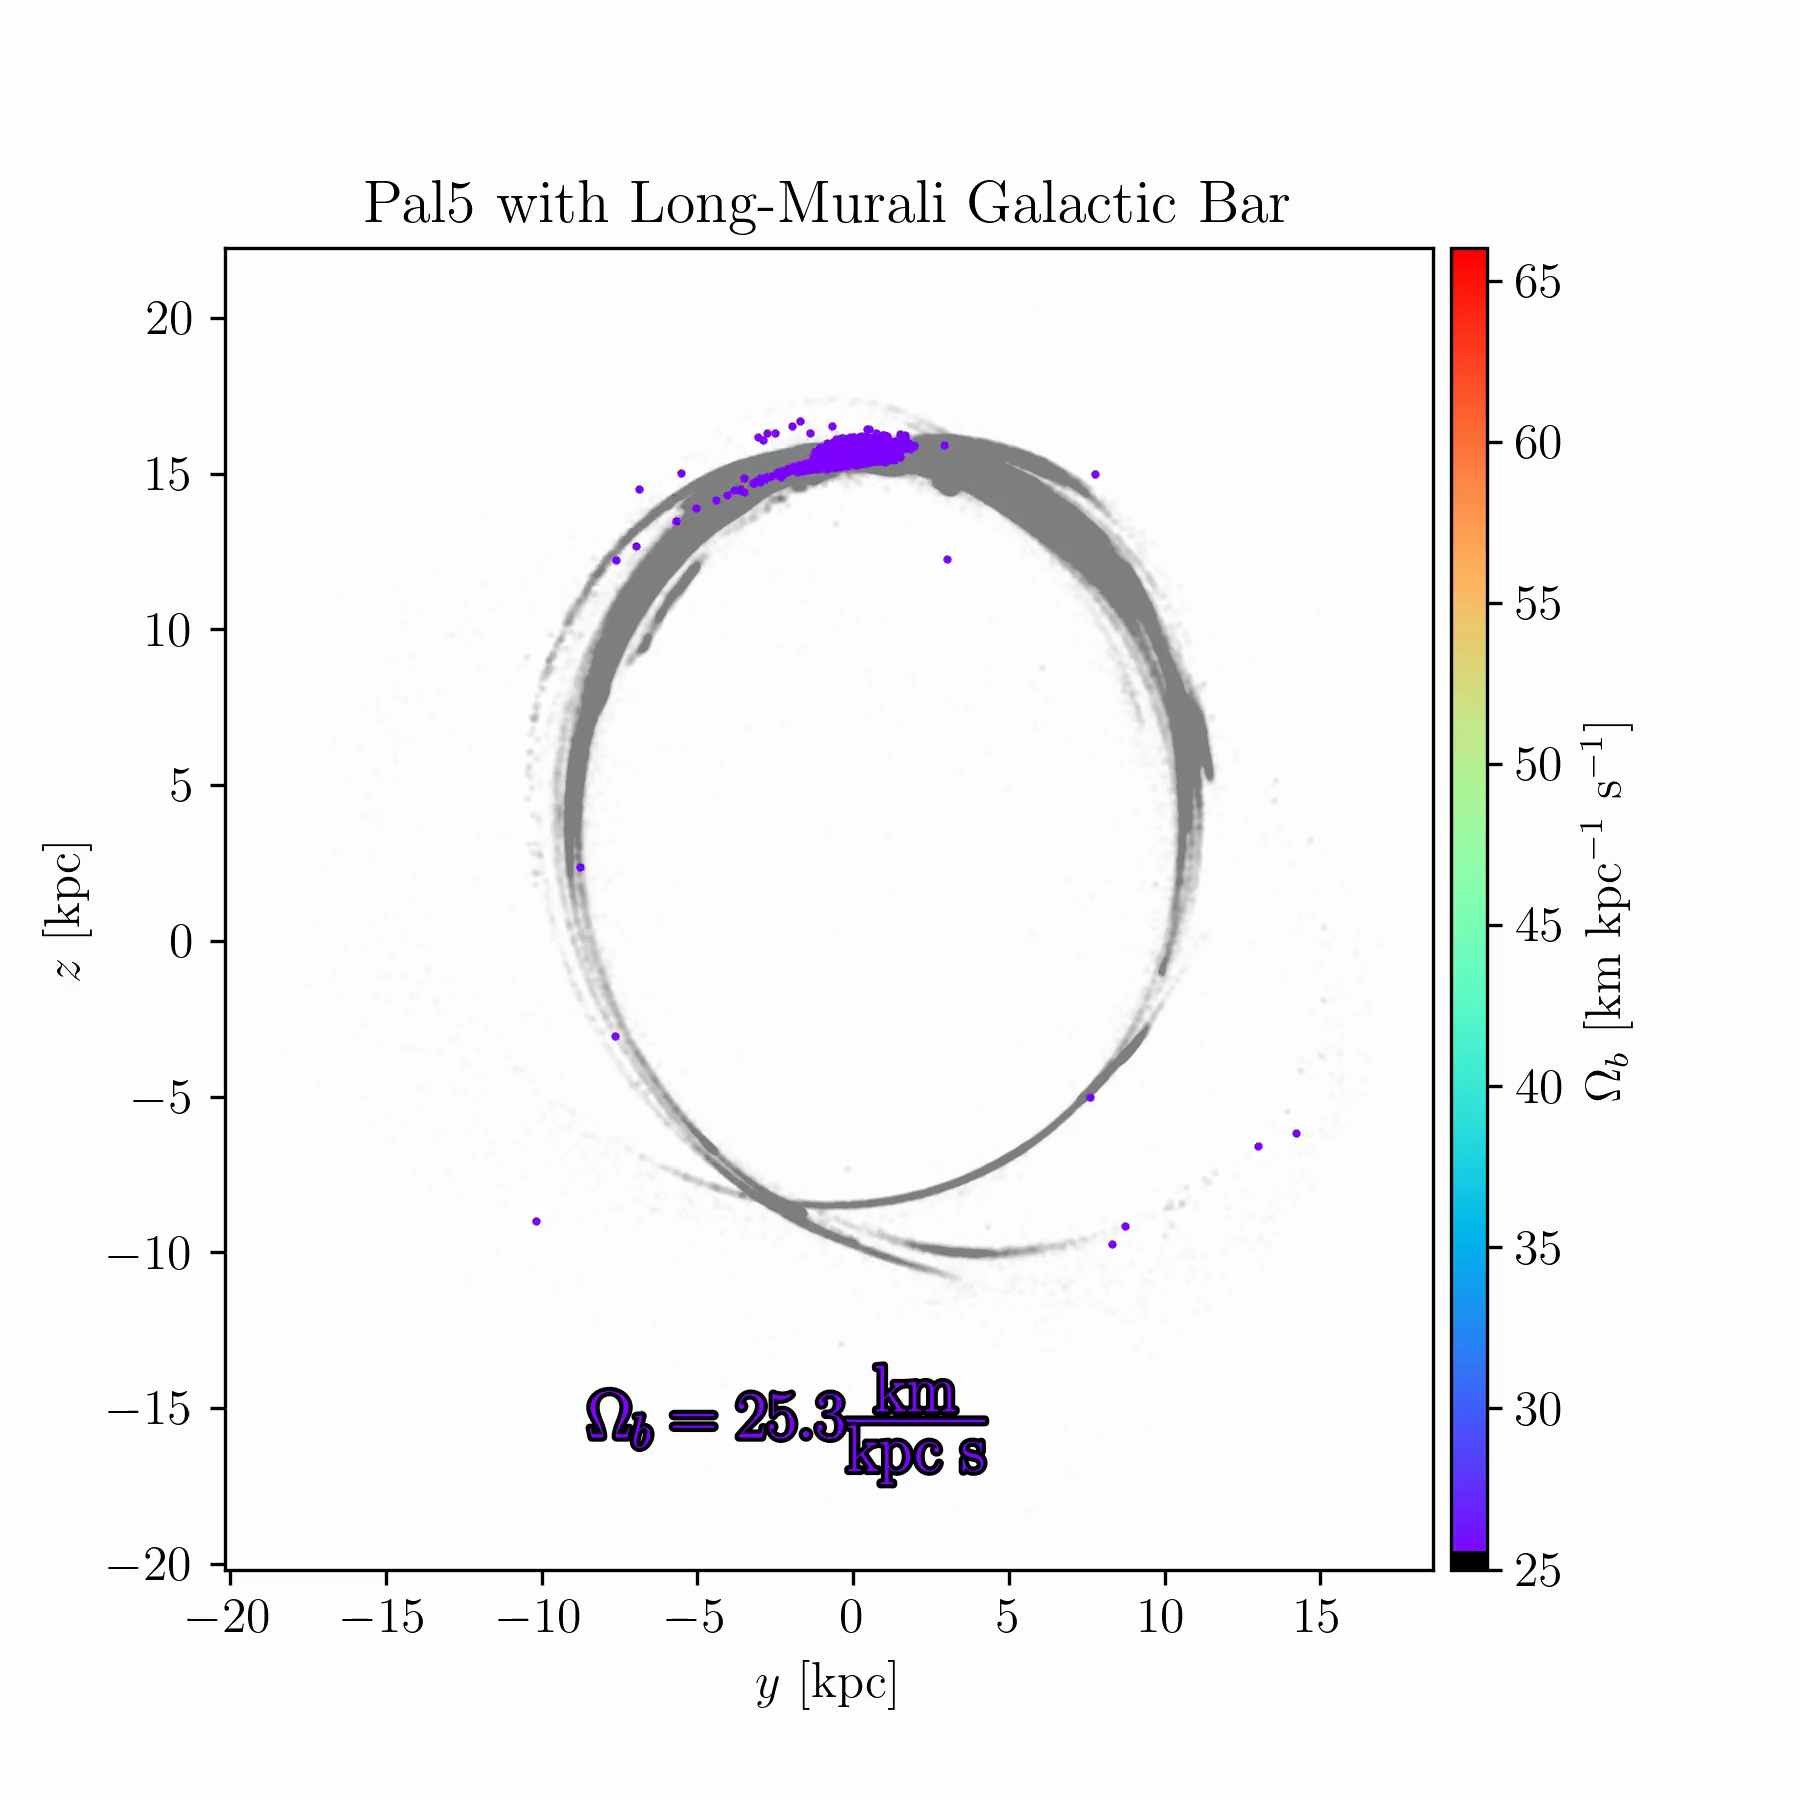
\includegraphics[width=.32\linewidth]{images/frame_0002.png}&
                    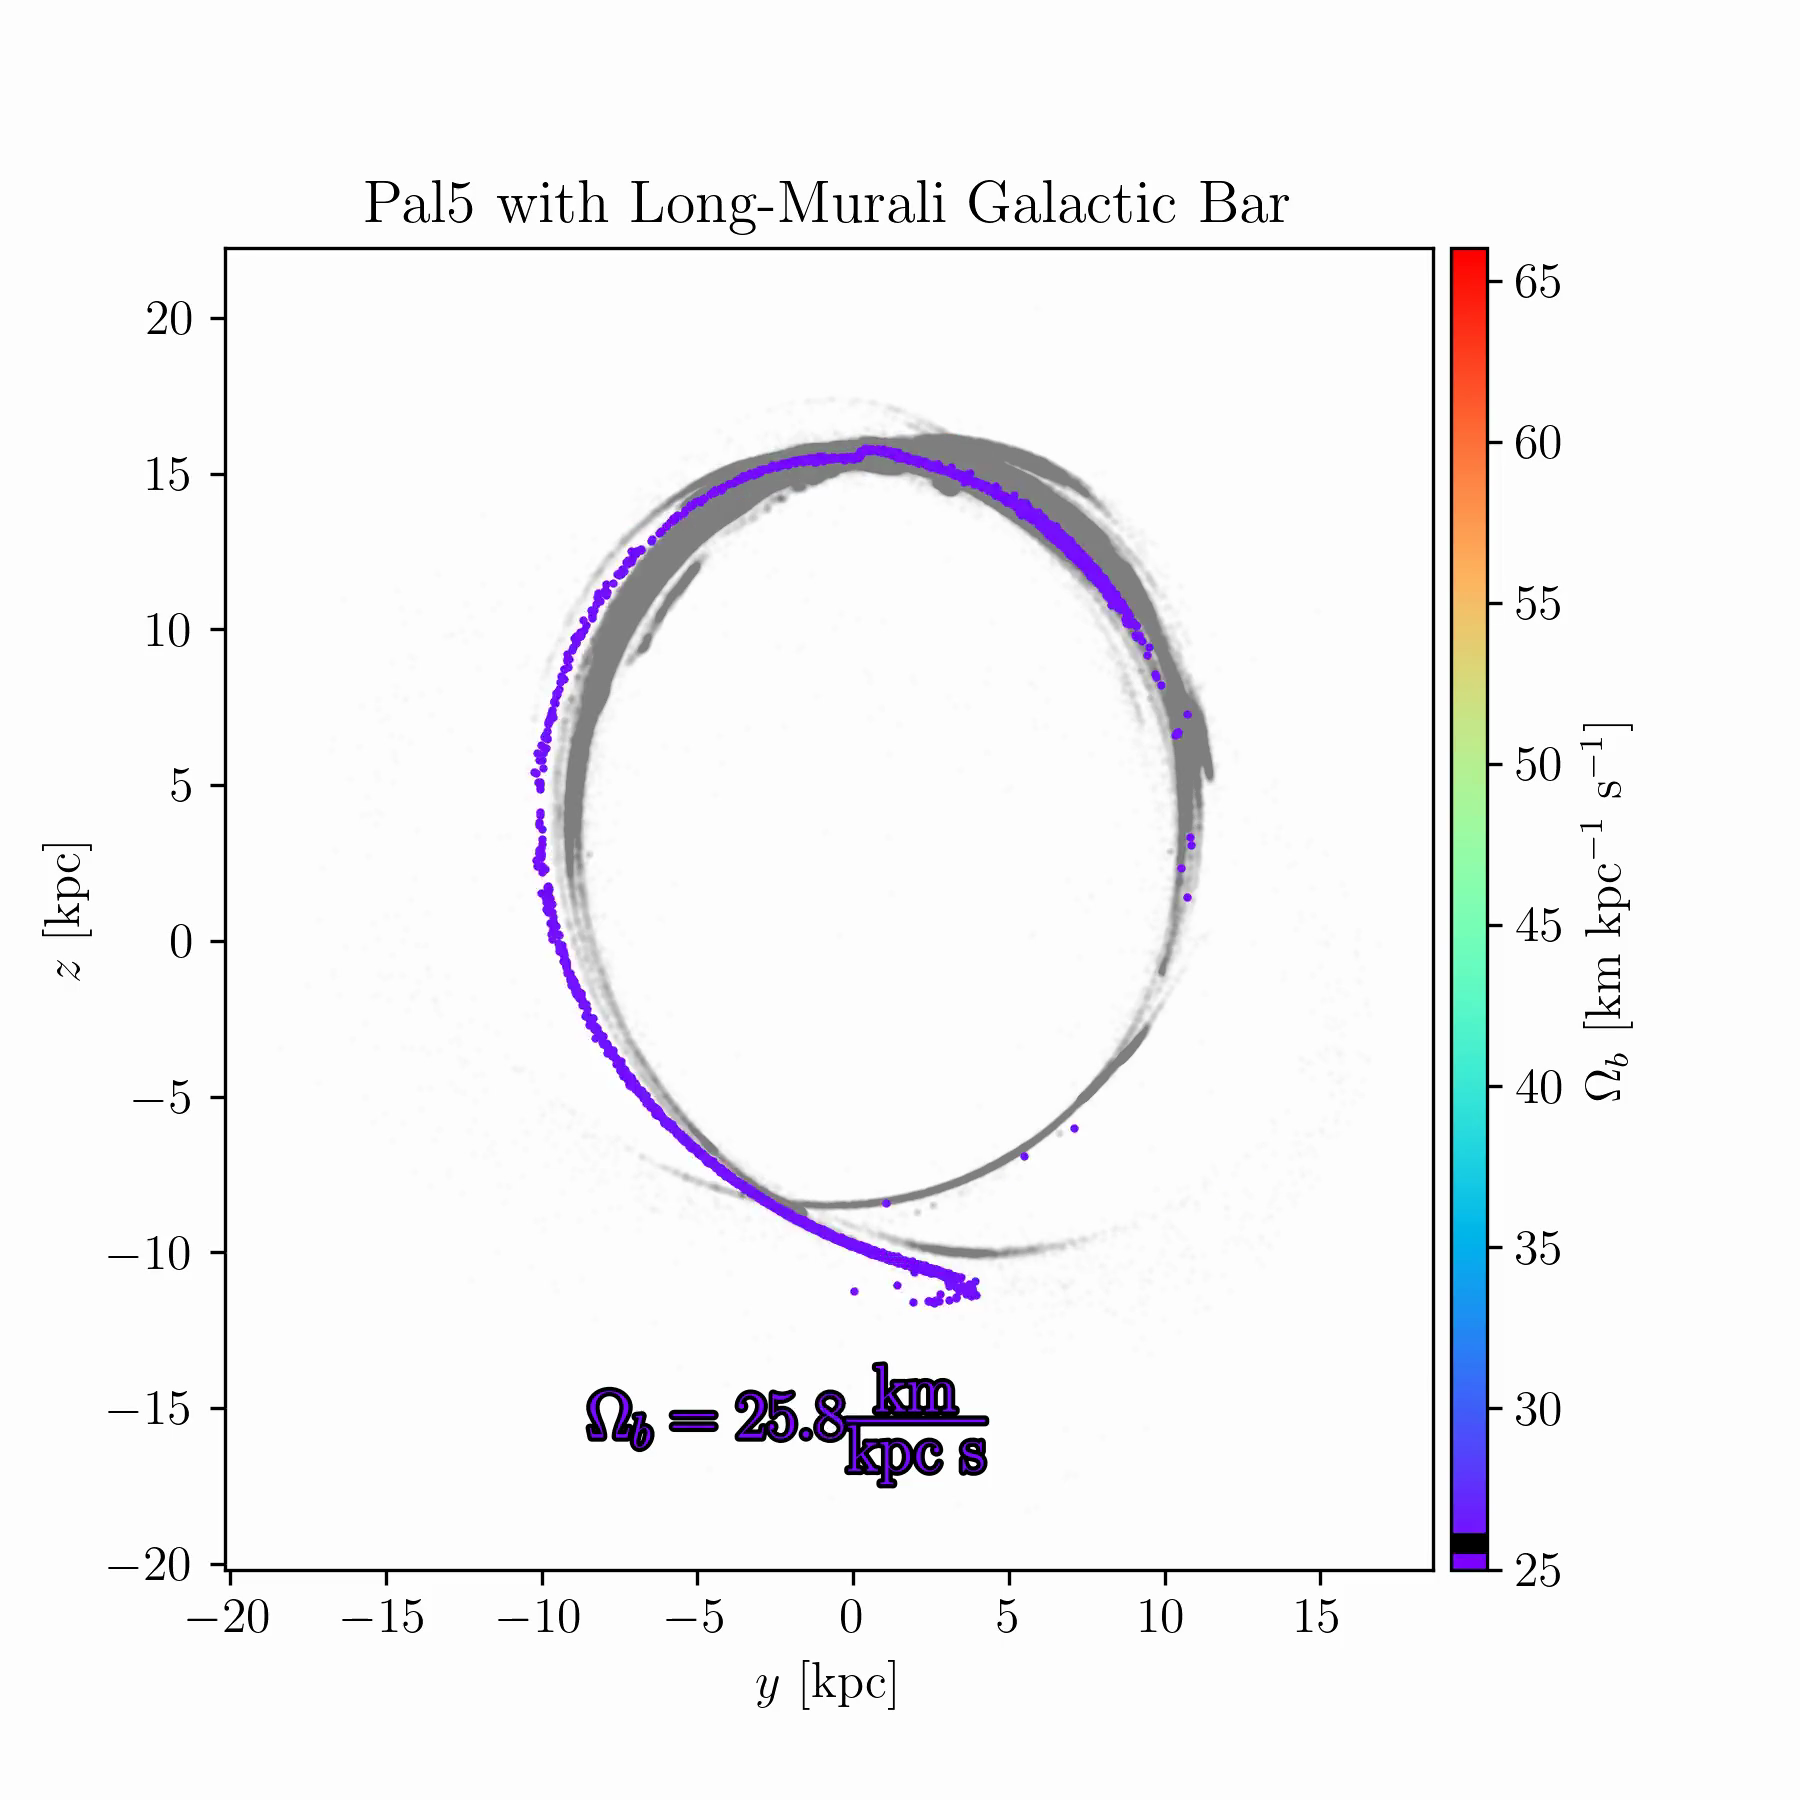
\includegraphics[width=.32\linewidth]{images/frame_0004.png}&
                    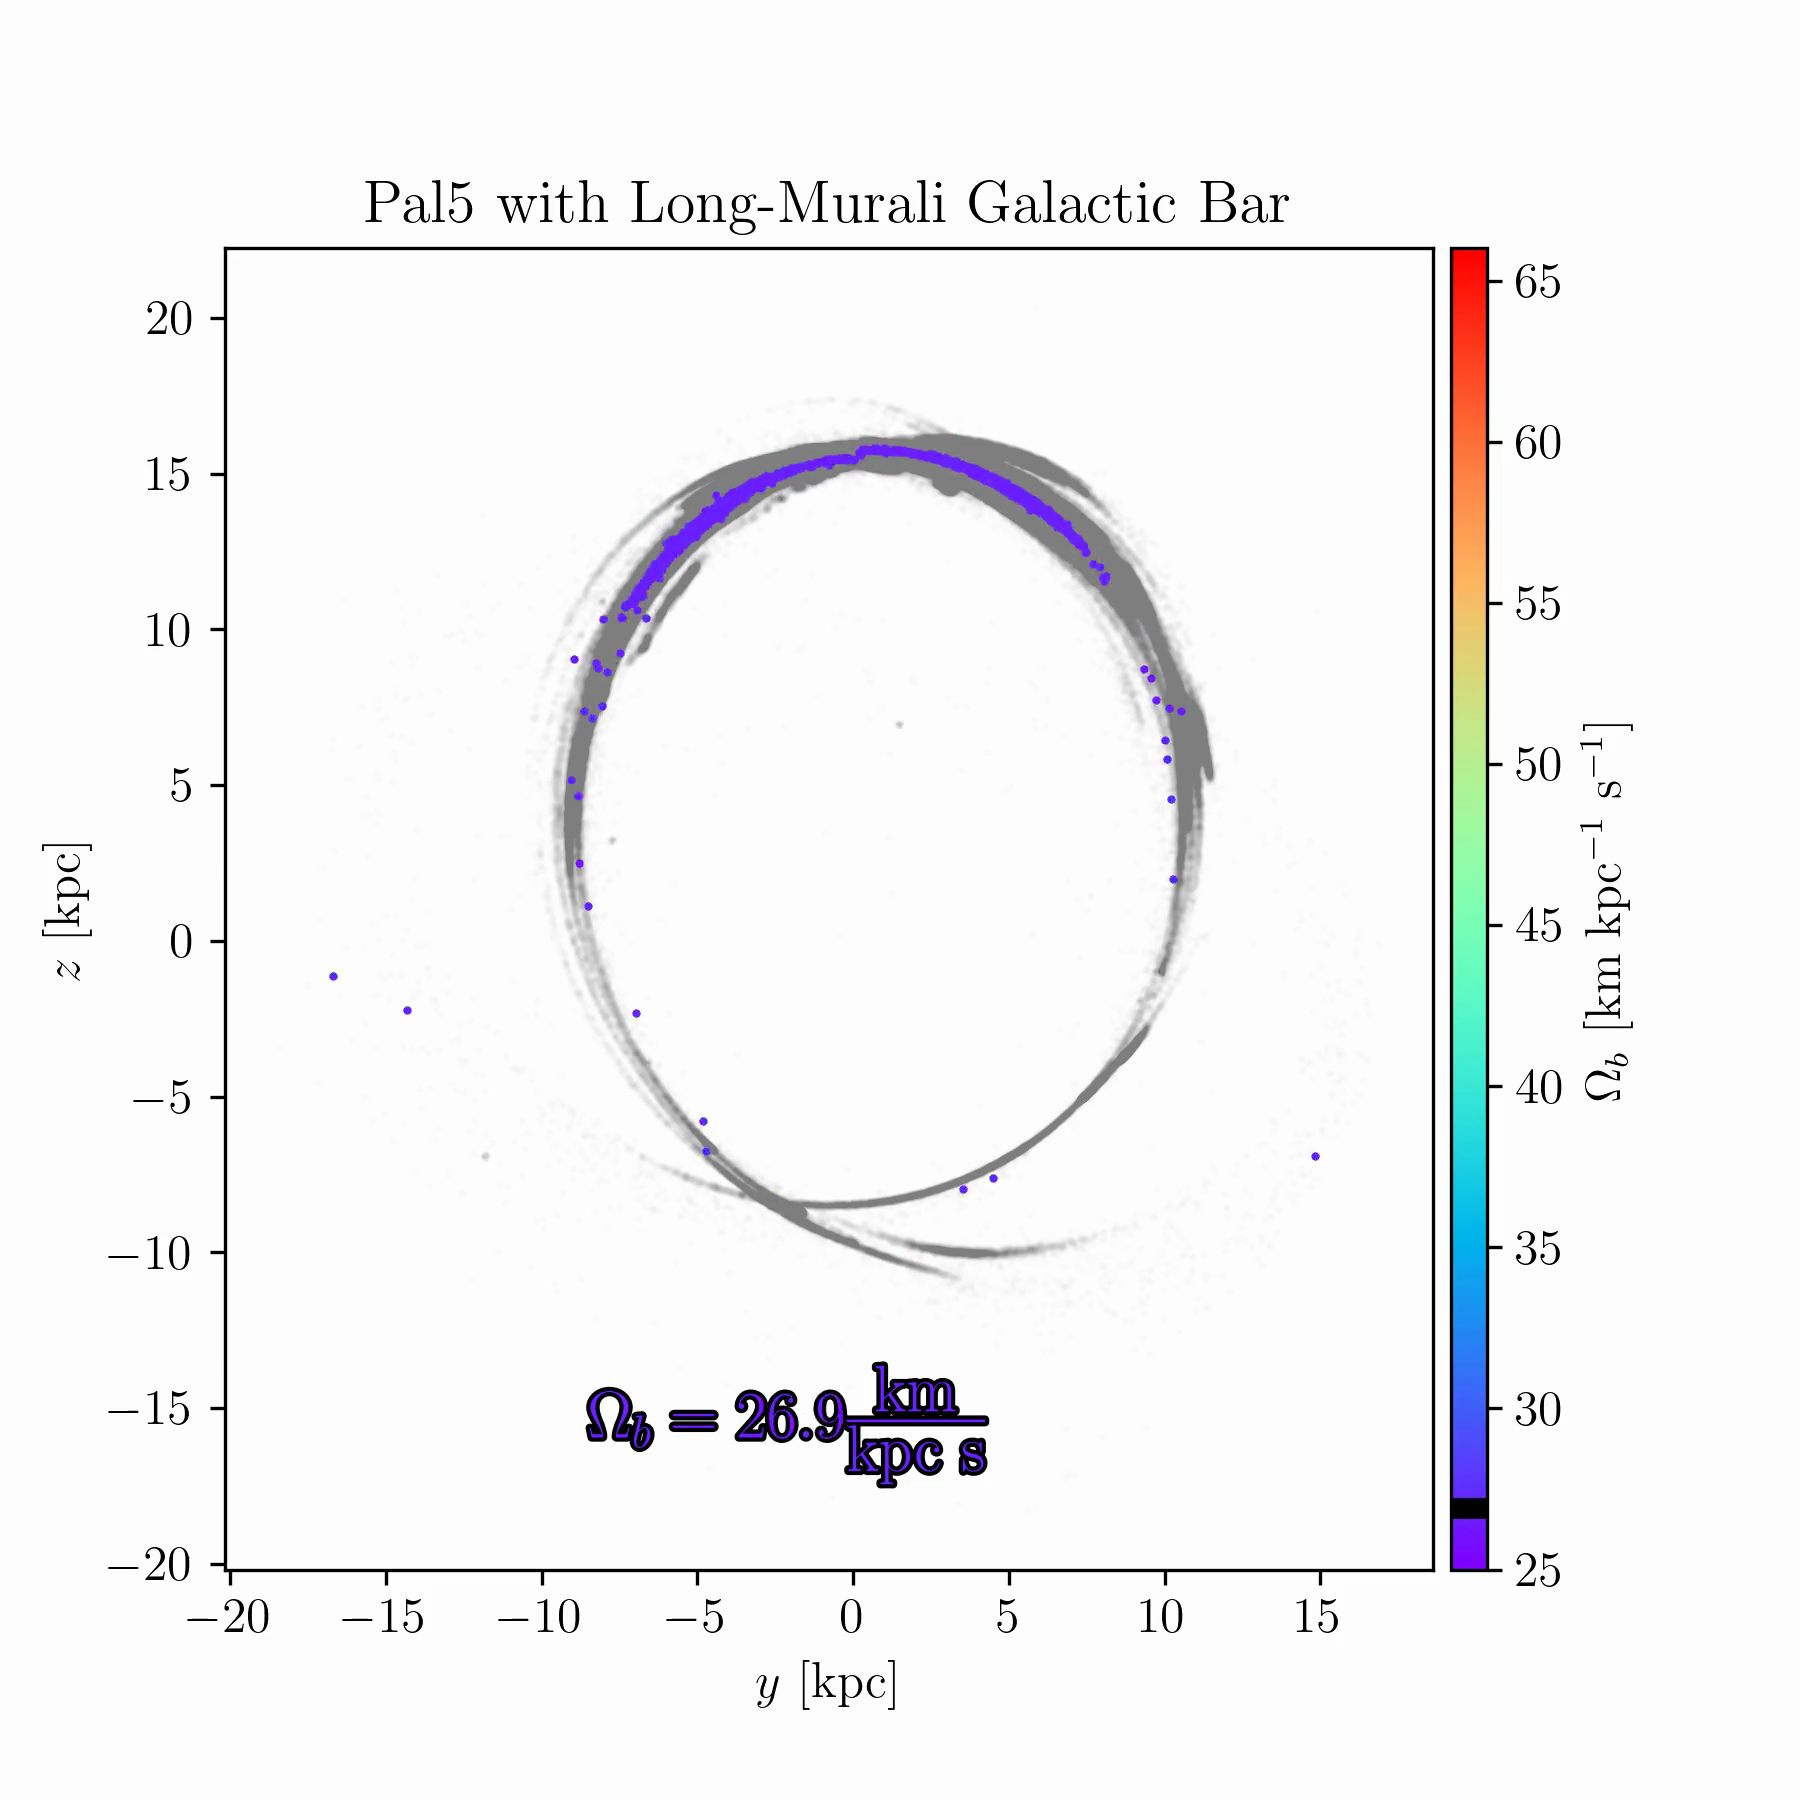
\includegraphics[width=.32\linewidth]{images/frame_0008.png}\\
                    
                    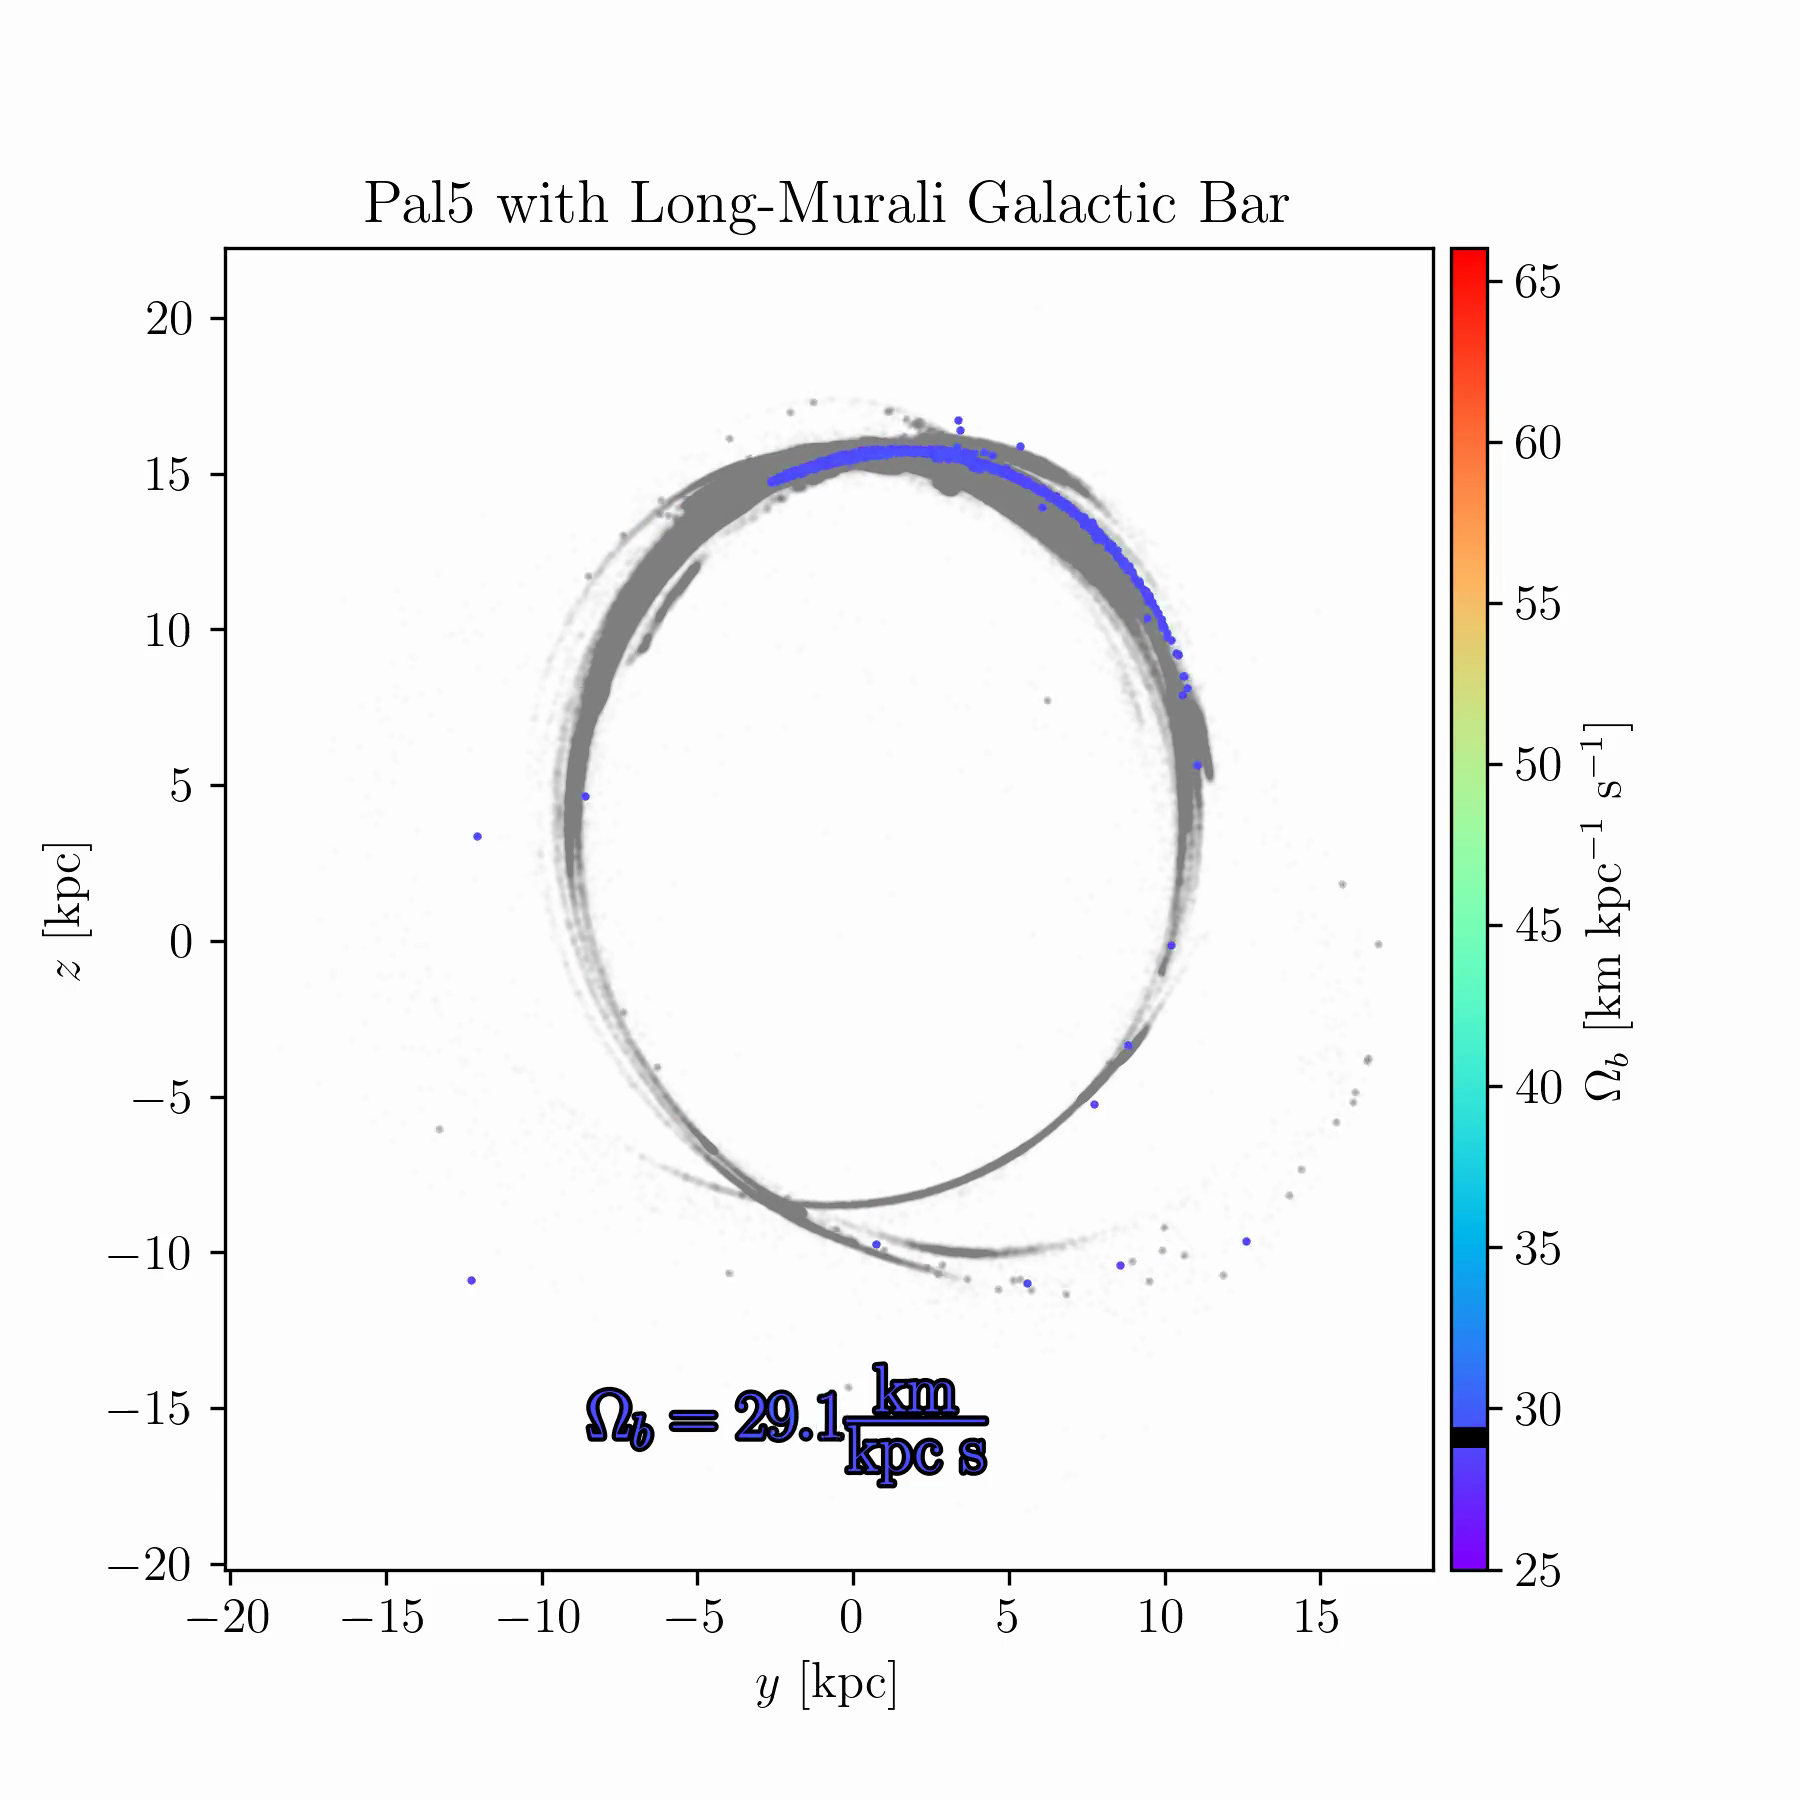
\includegraphics[width=.32\linewidth]{images/frame_0016.png}&
                    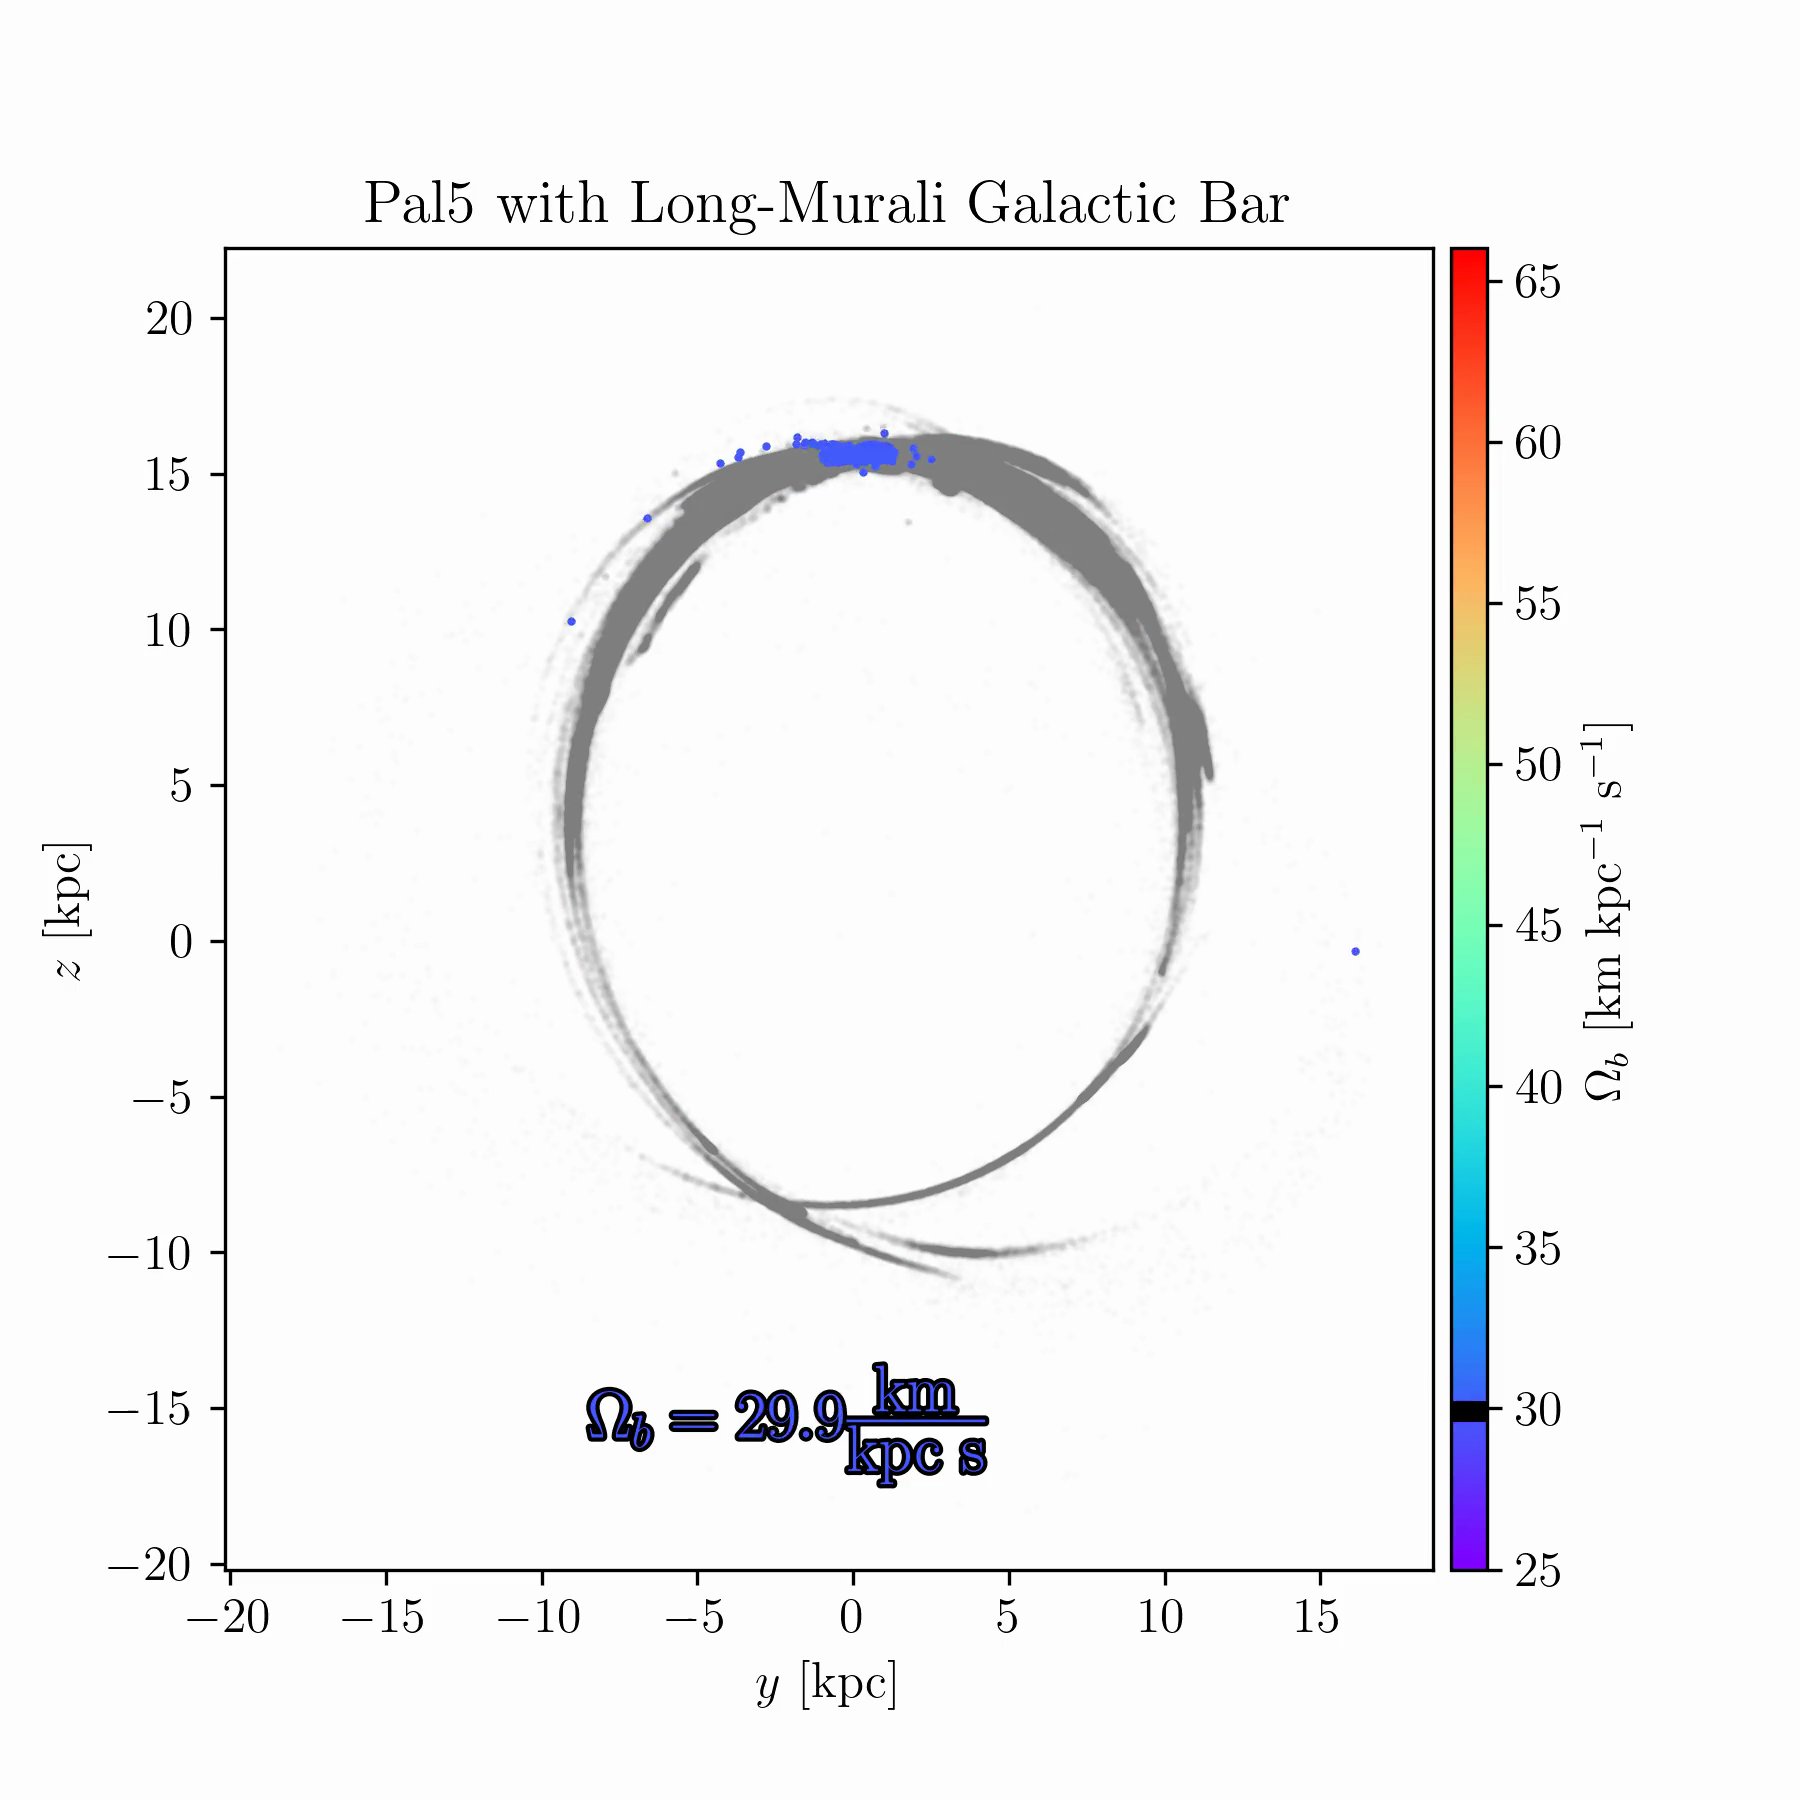
\includegraphics[width=.32\linewidth]{images/frame_0019.png}&
                    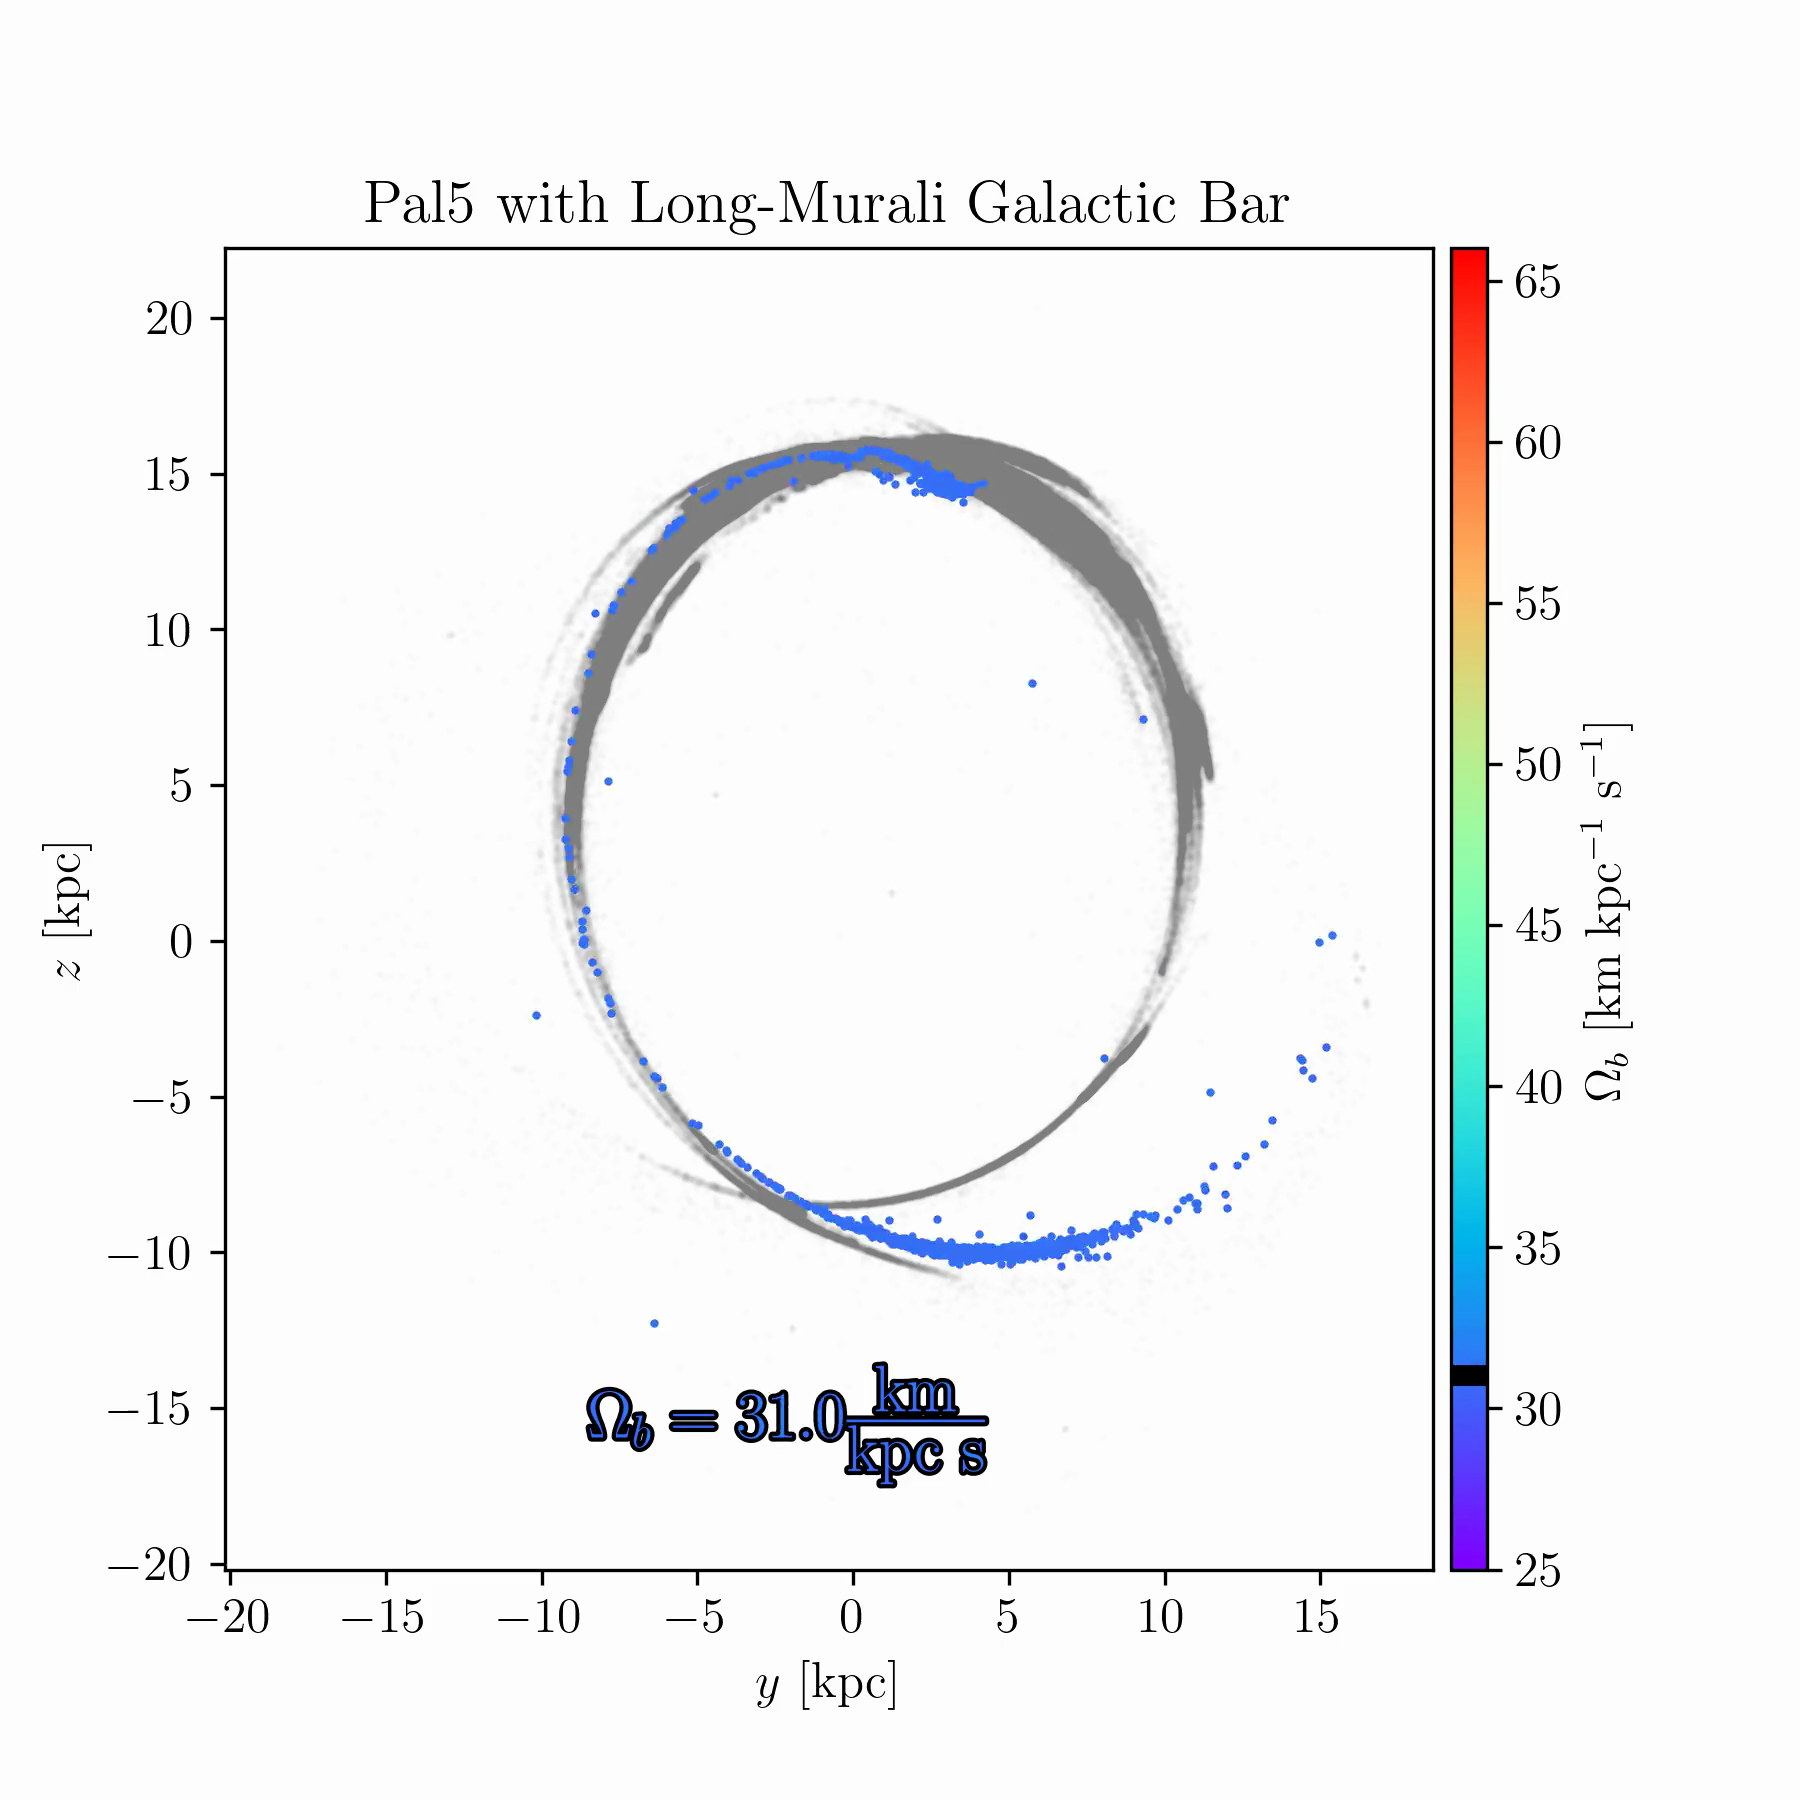
\includegraphics[width=.32\linewidth]{images/frame_0023.png}\\
                    
                    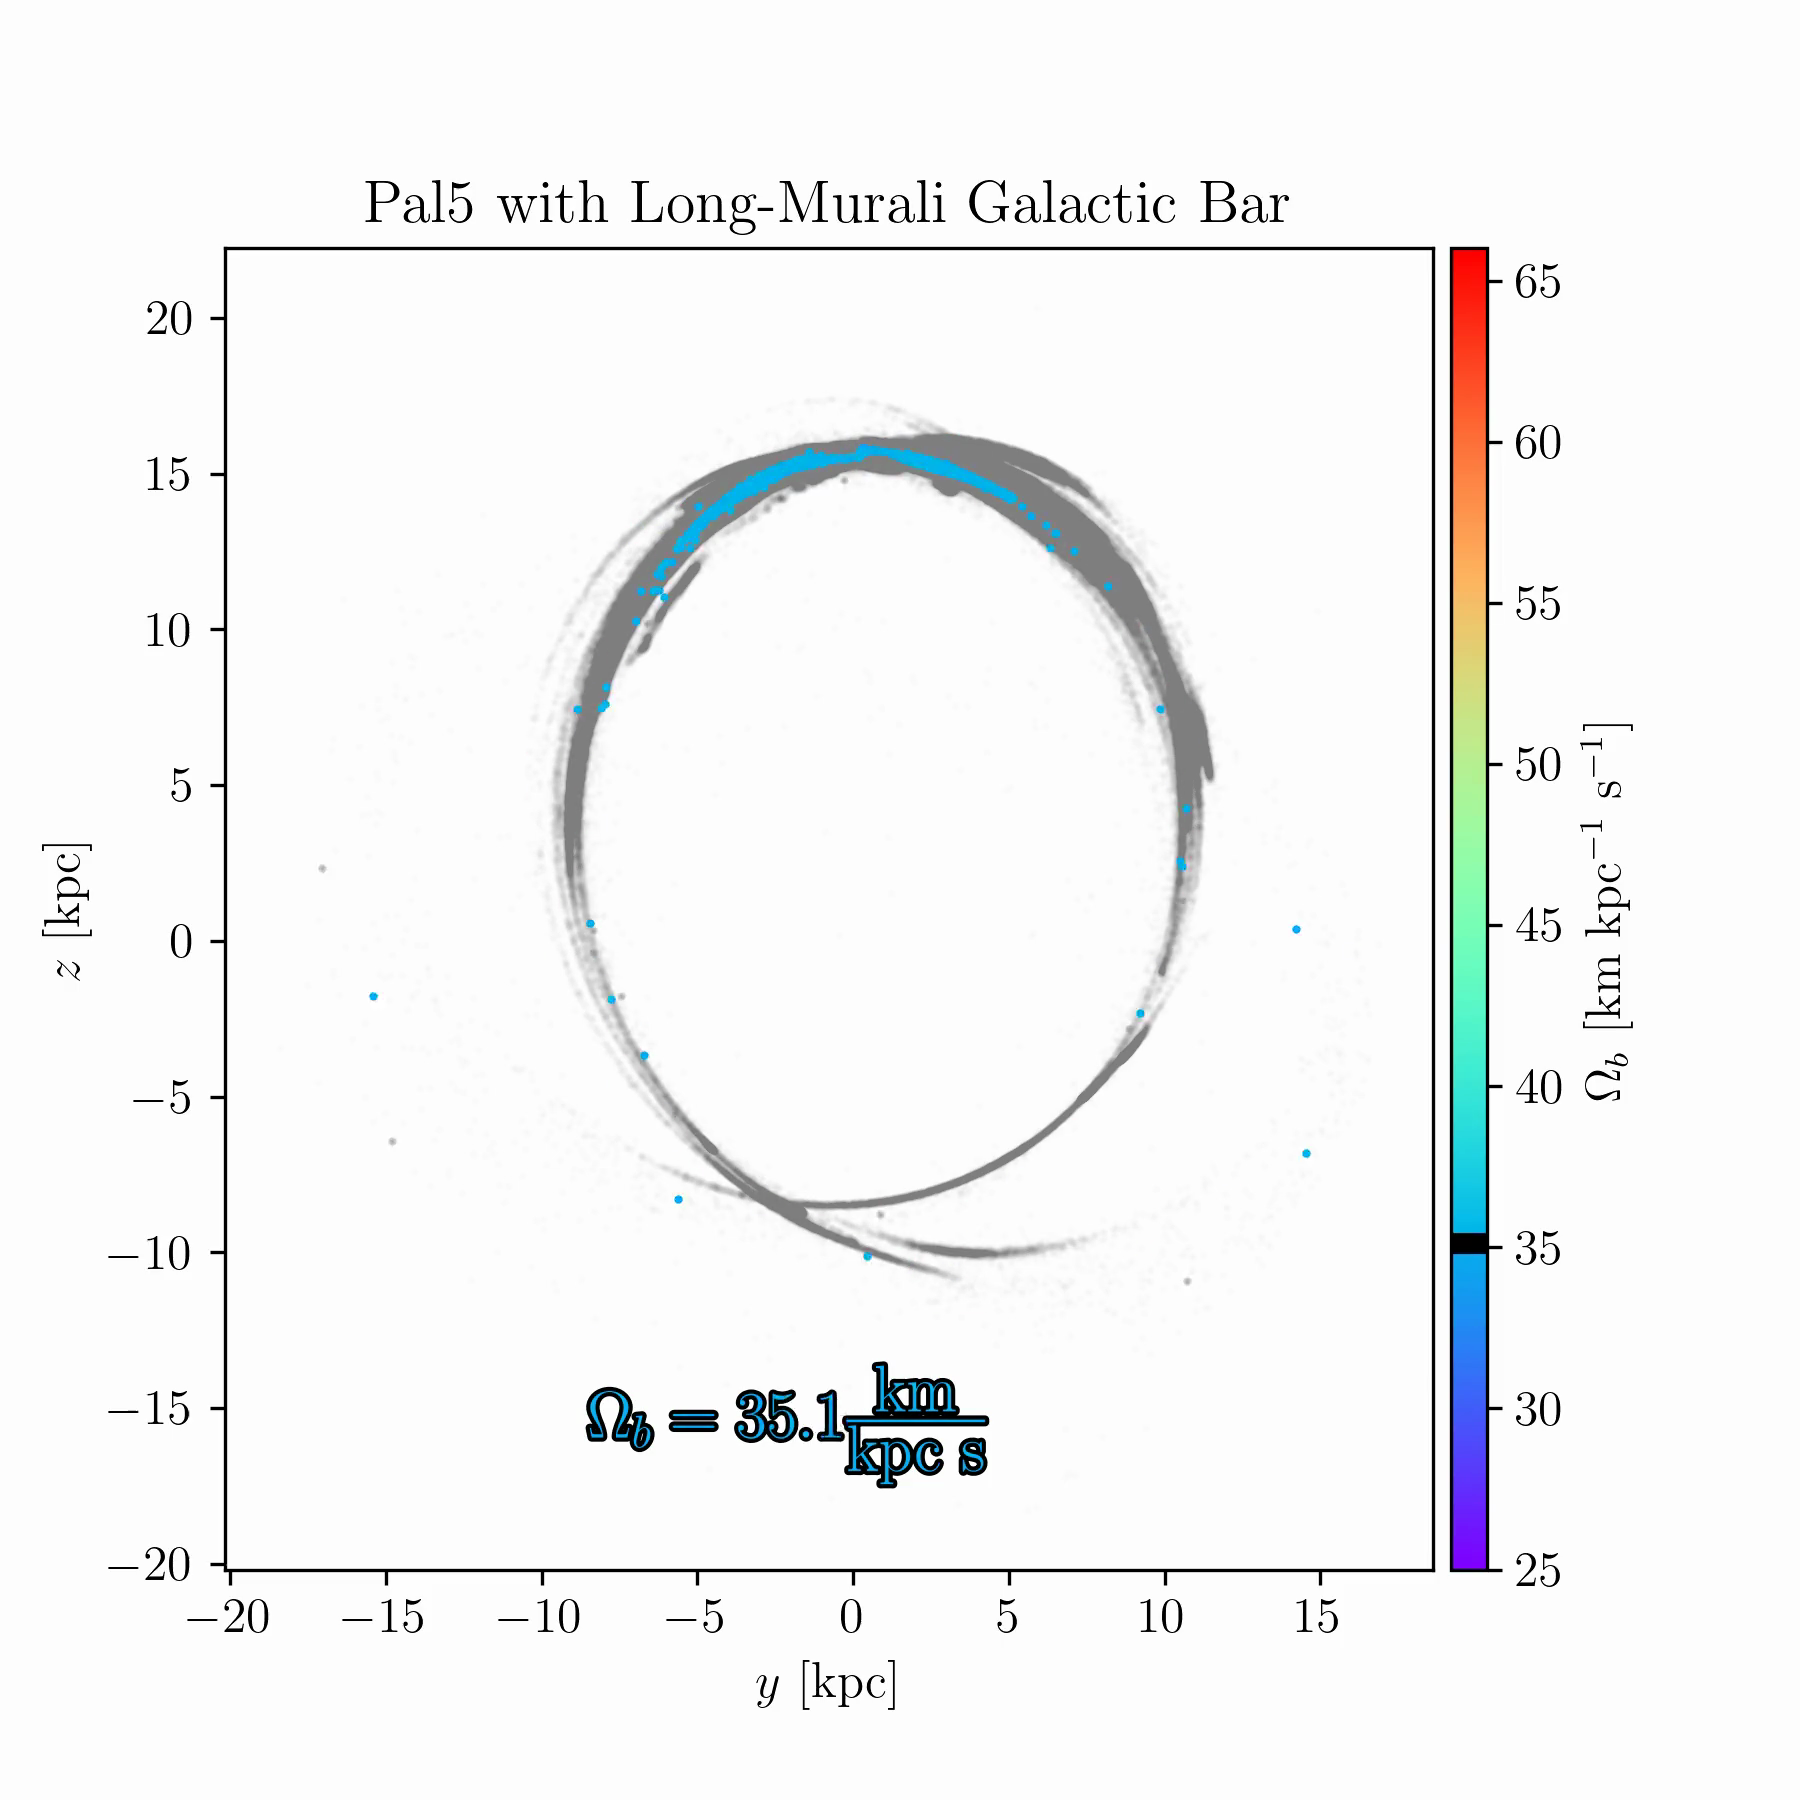
\includegraphics[width=.32\linewidth]{images/frame_0038.png}&
                    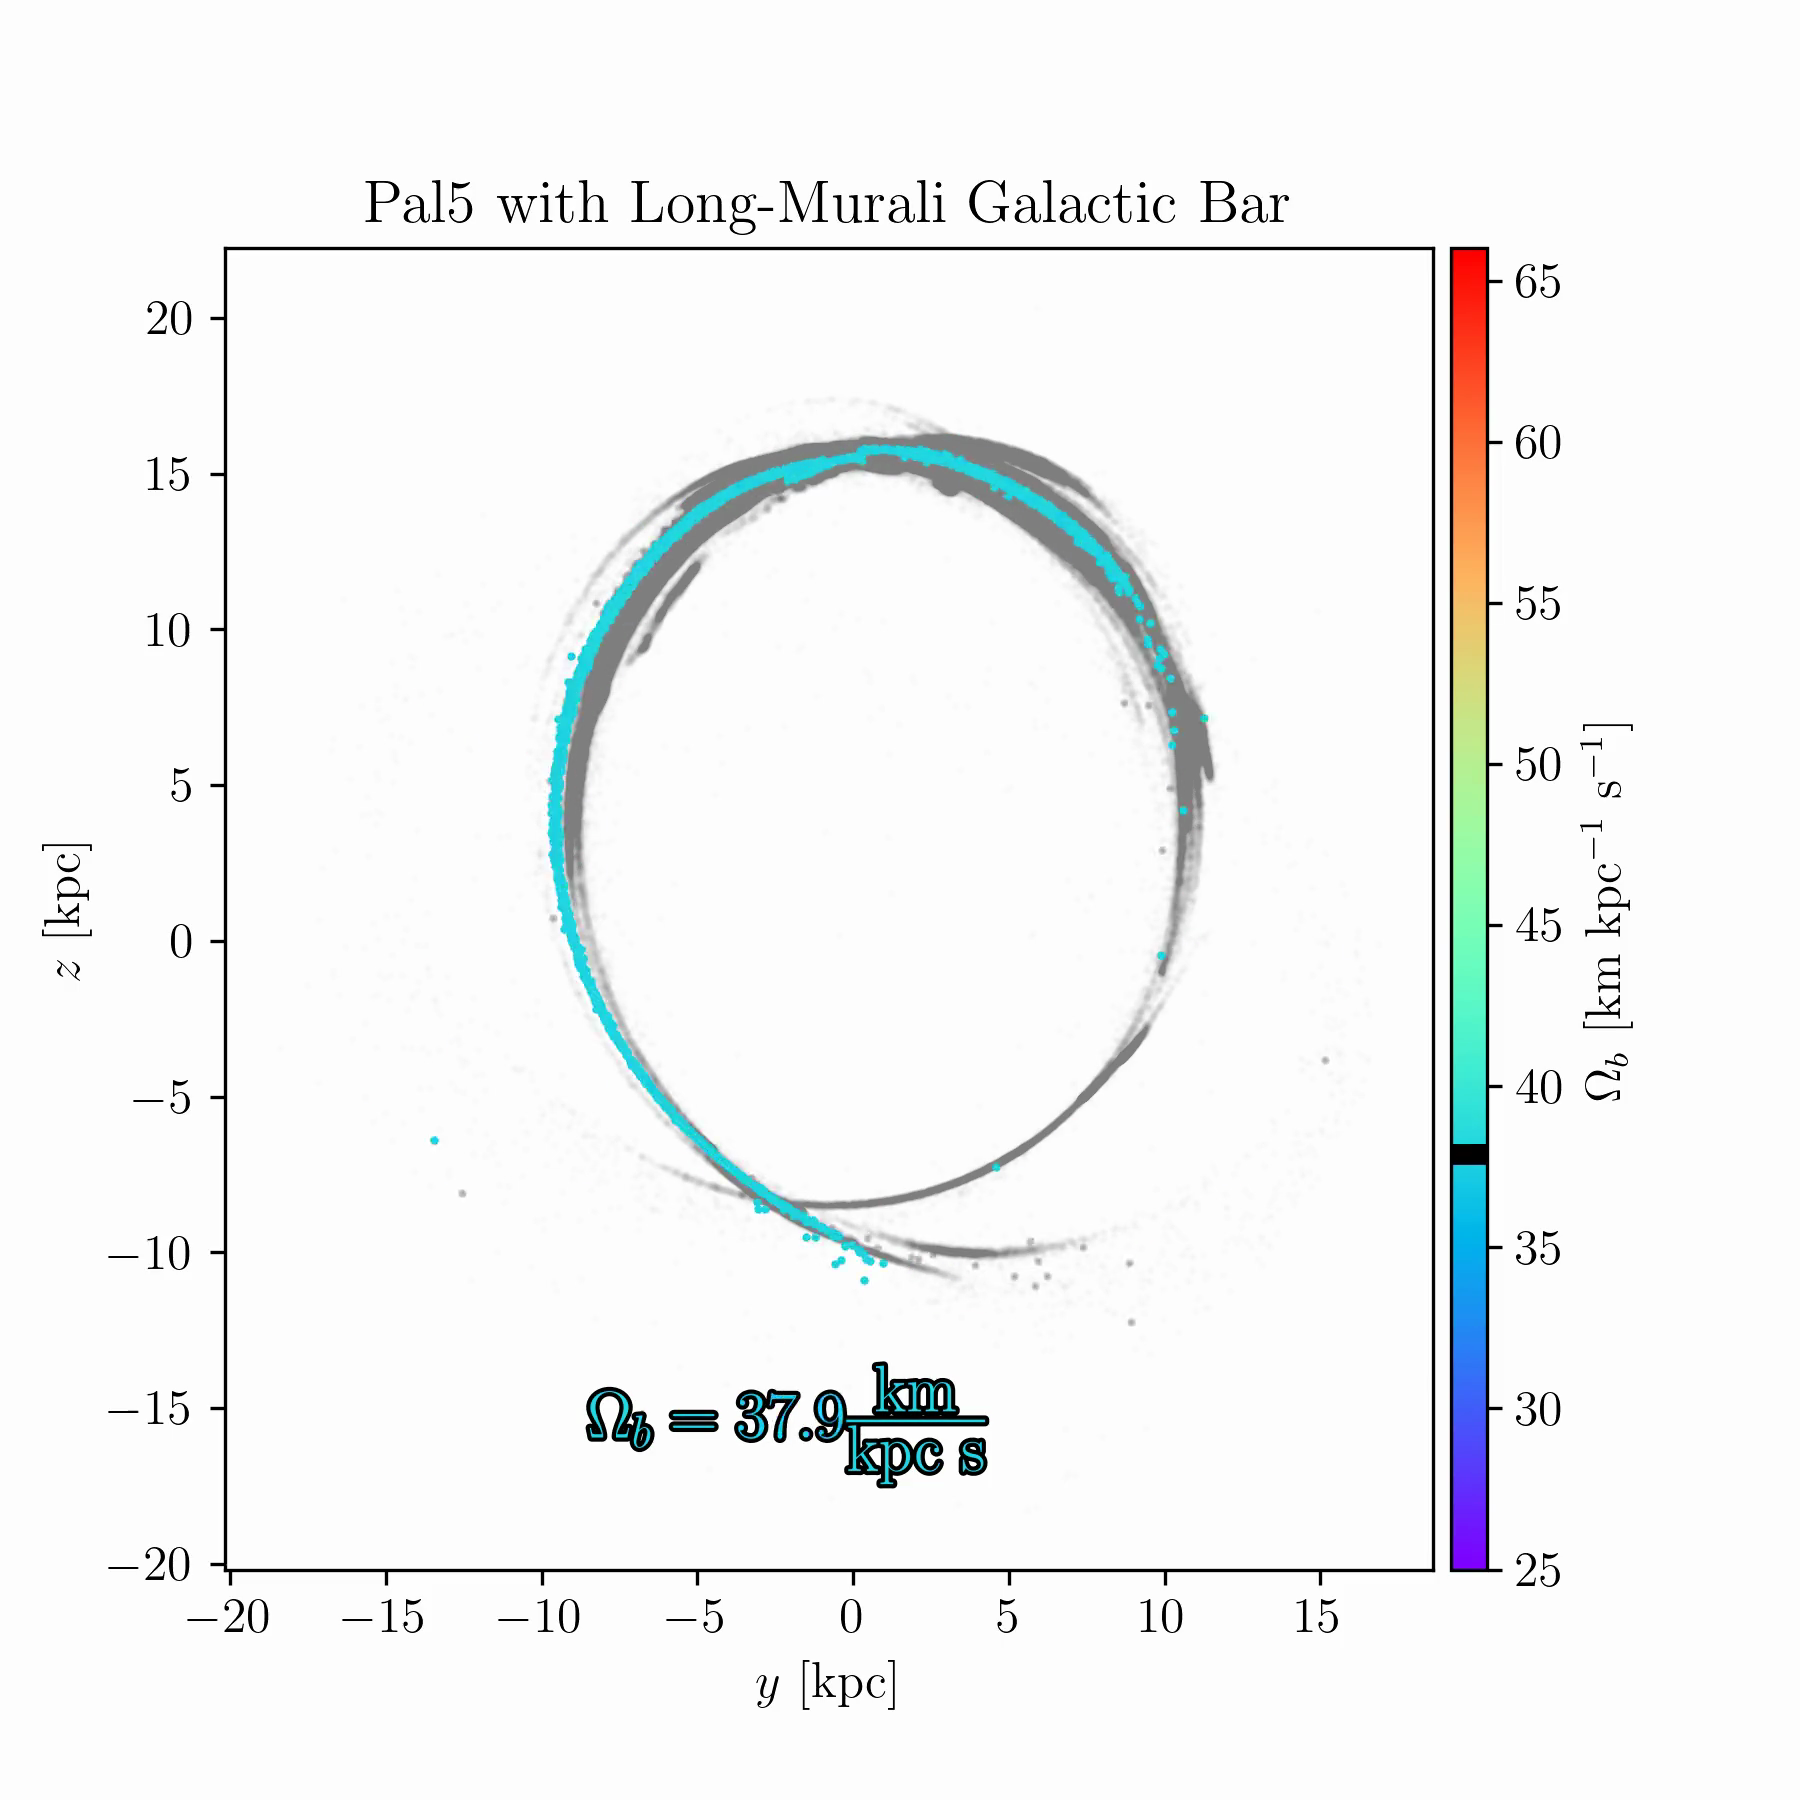
\includegraphics[width=.32\linewidth]{images/frame_0048.png}&
                    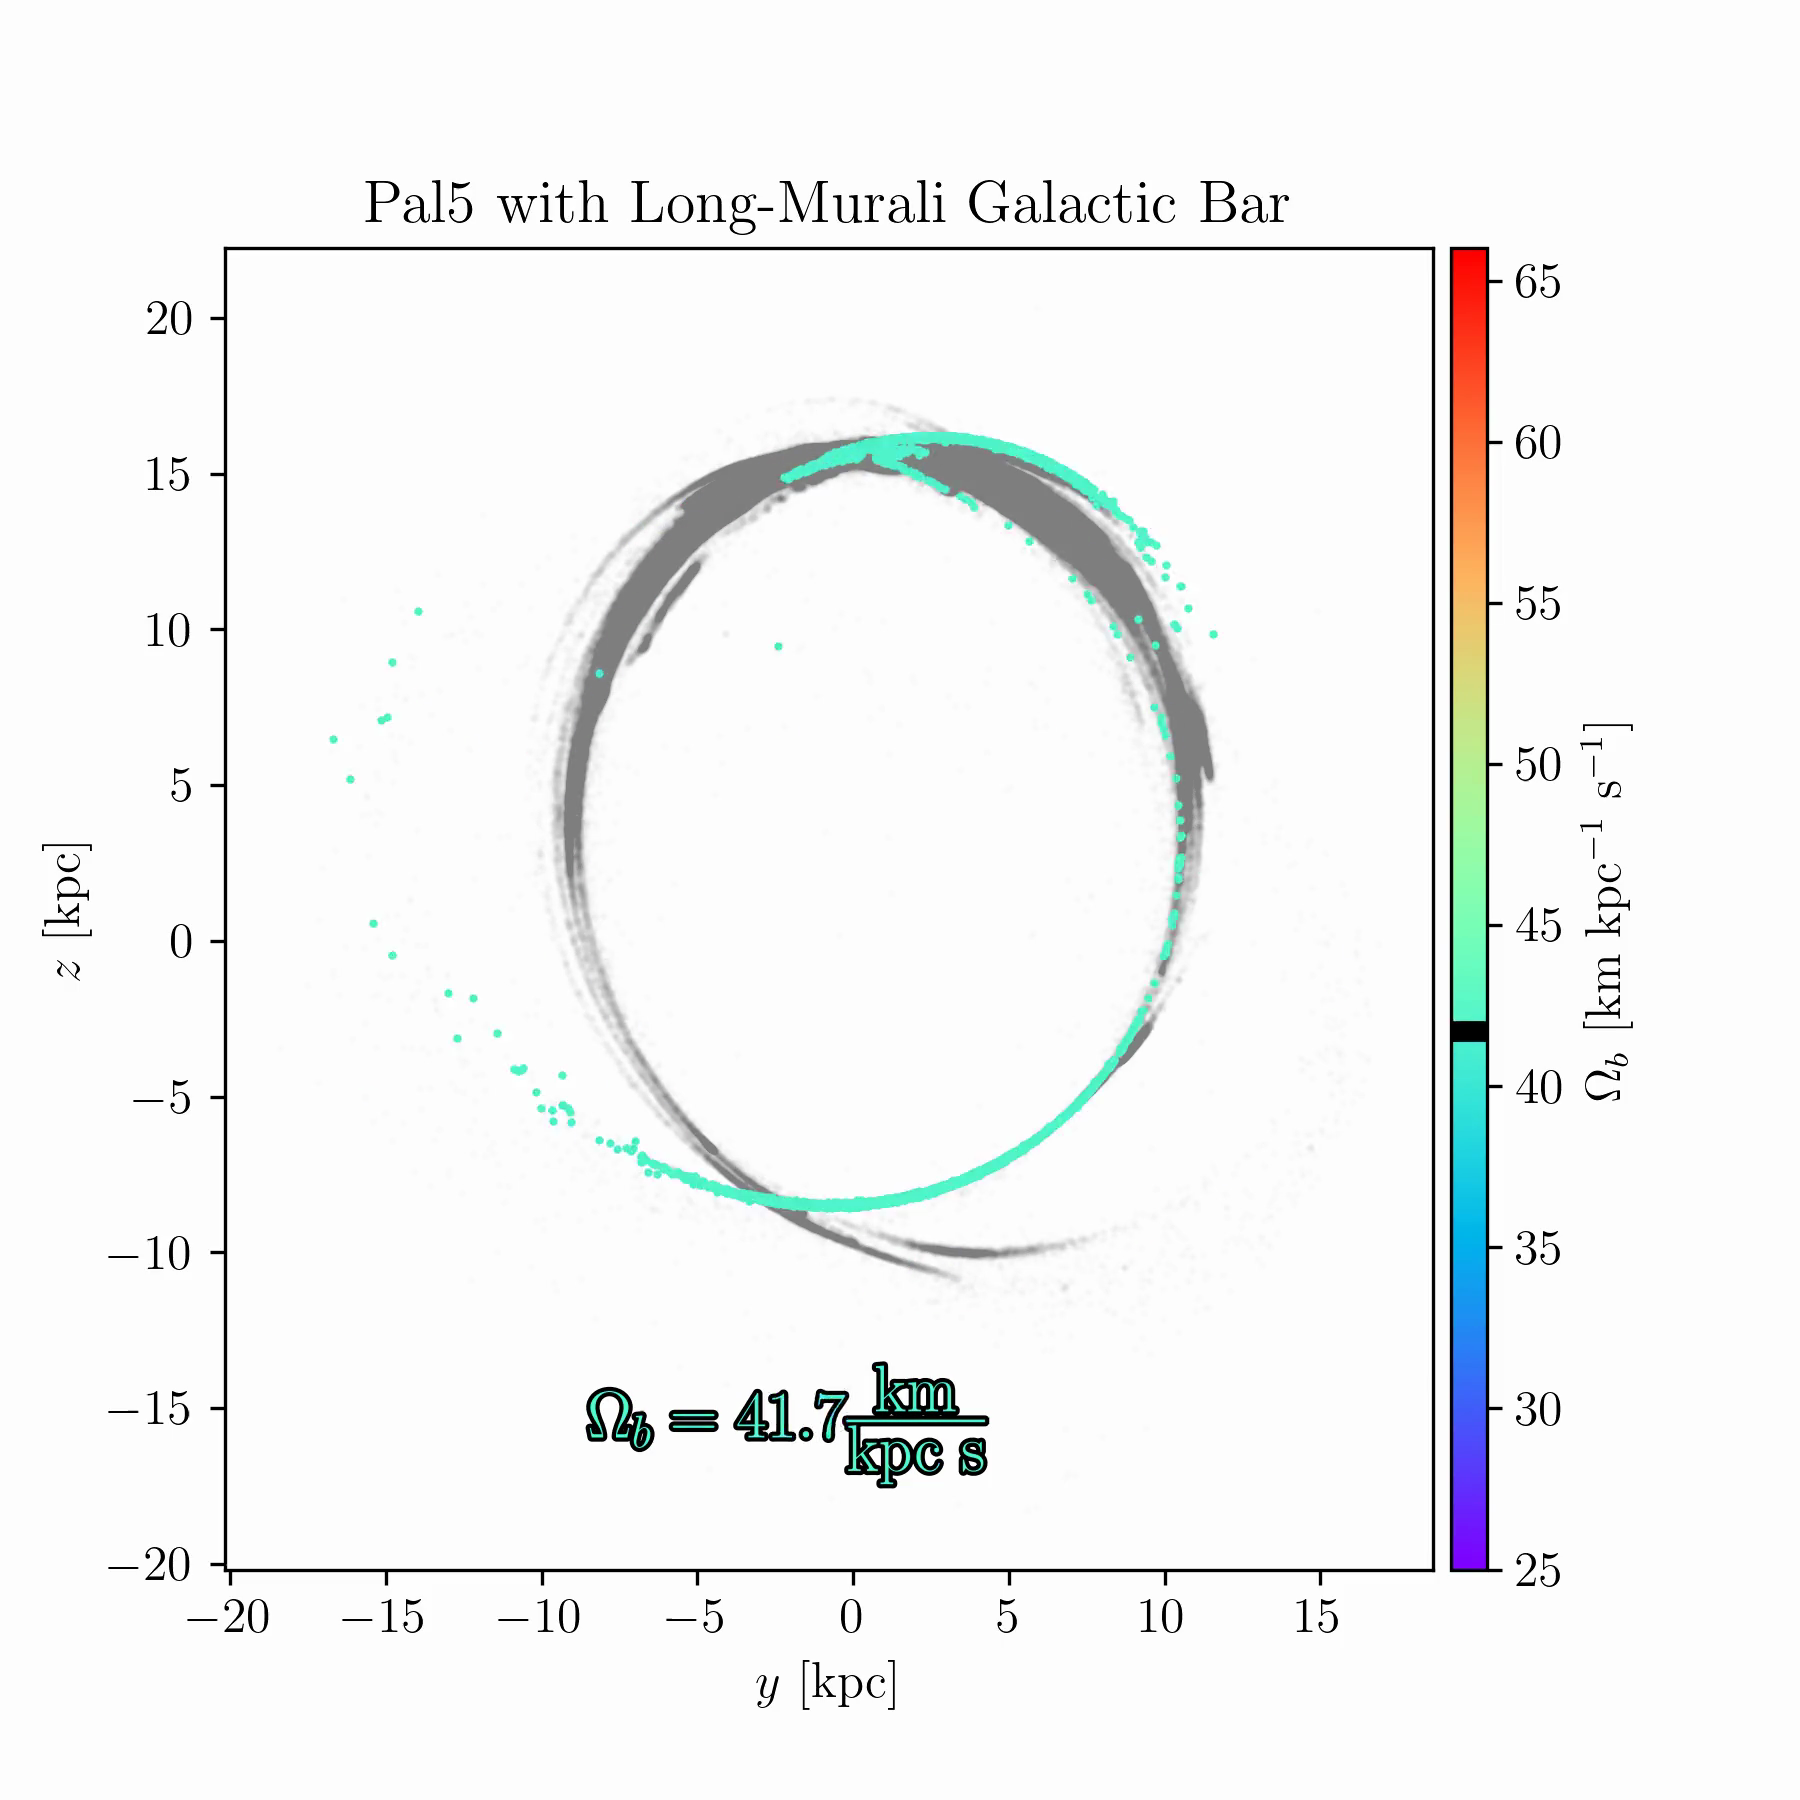
\includegraphics[width=.32\linewidth]{images/frame_0062.png}\\
                    
                    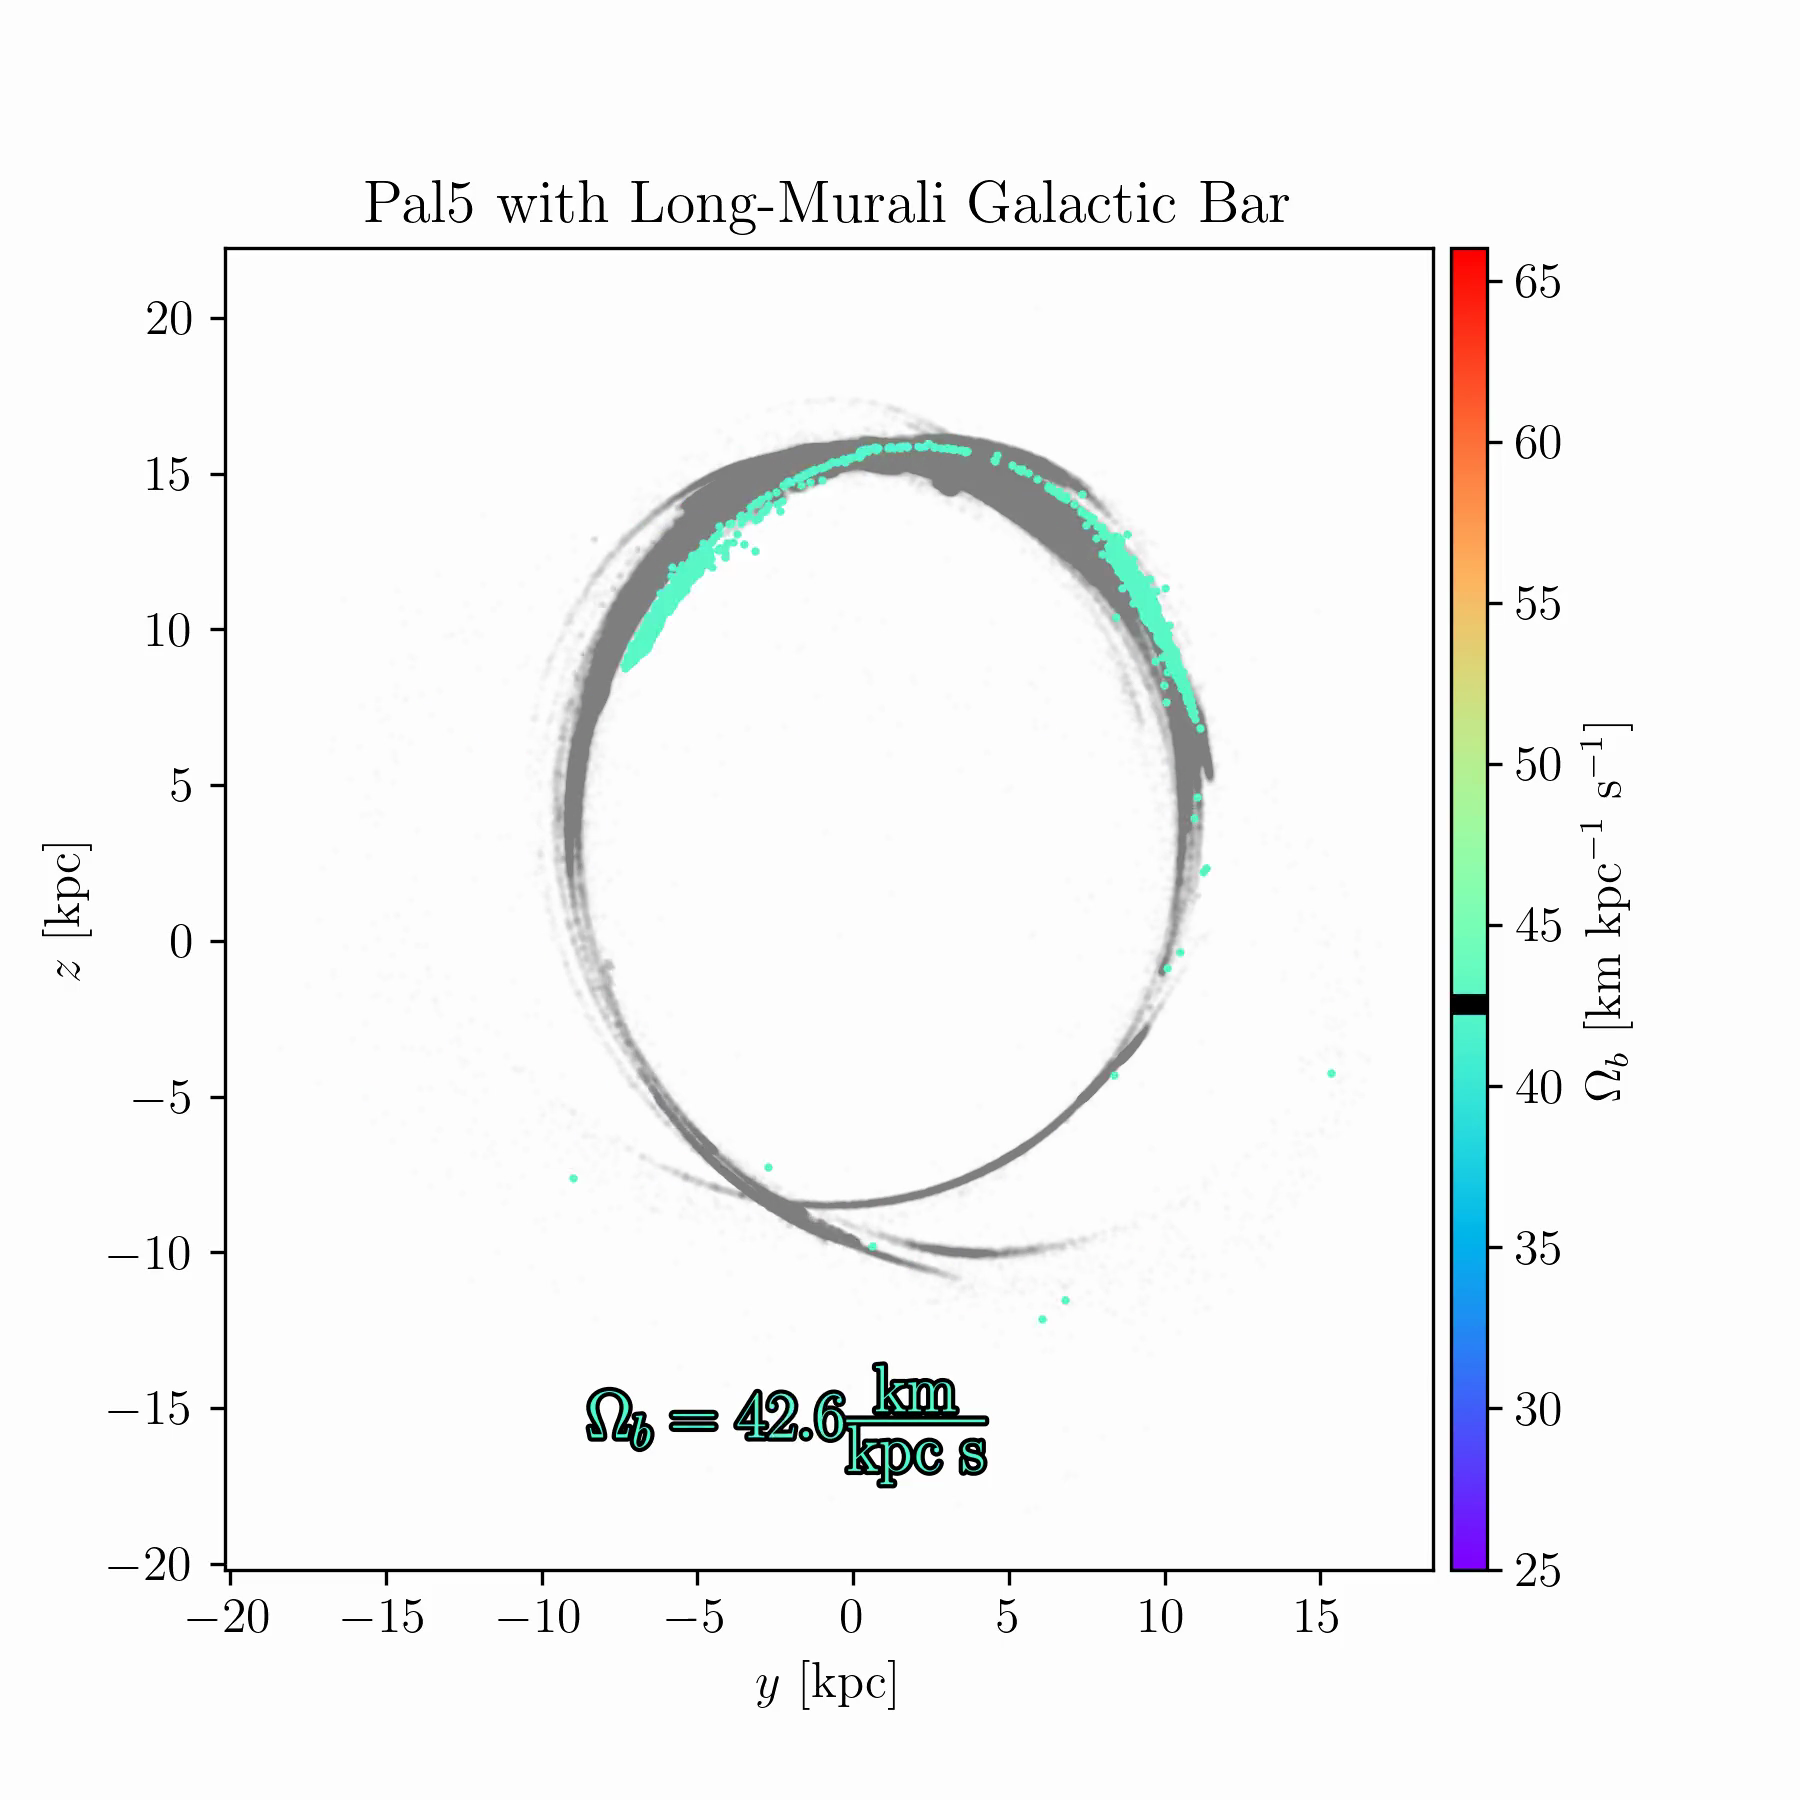
\includegraphics[width=.32\linewidth]{images/frame_0065.png}&
                    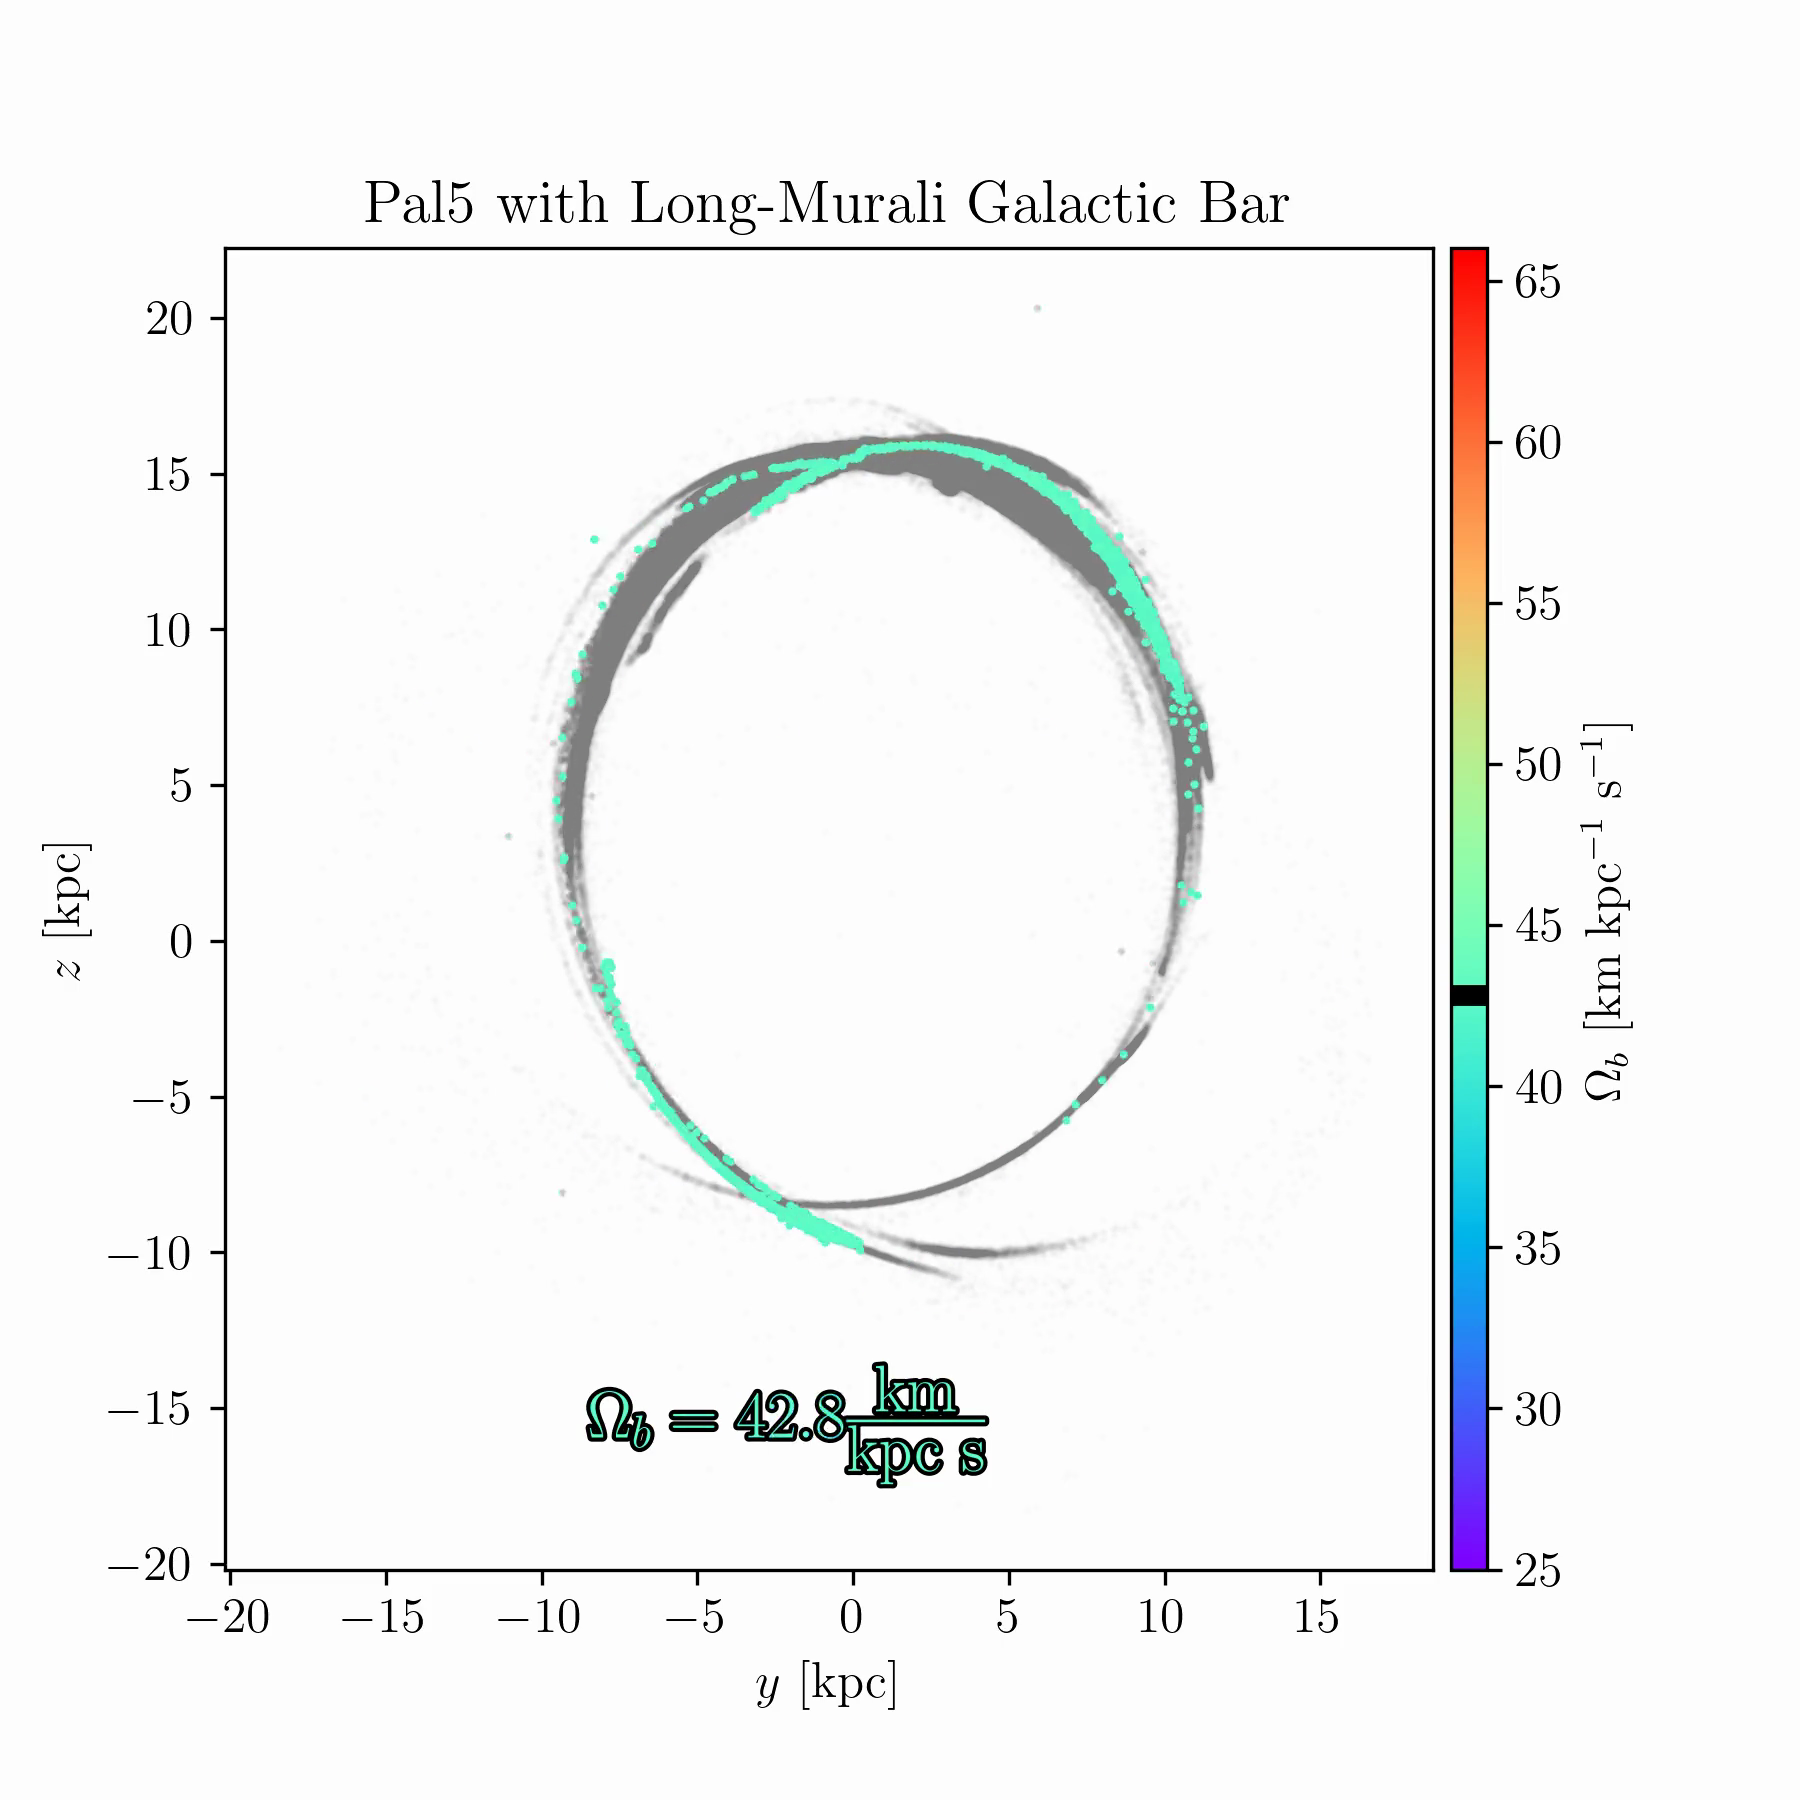
\includegraphics[width=.32\linewidth]{images/frame_0066.png}&
                    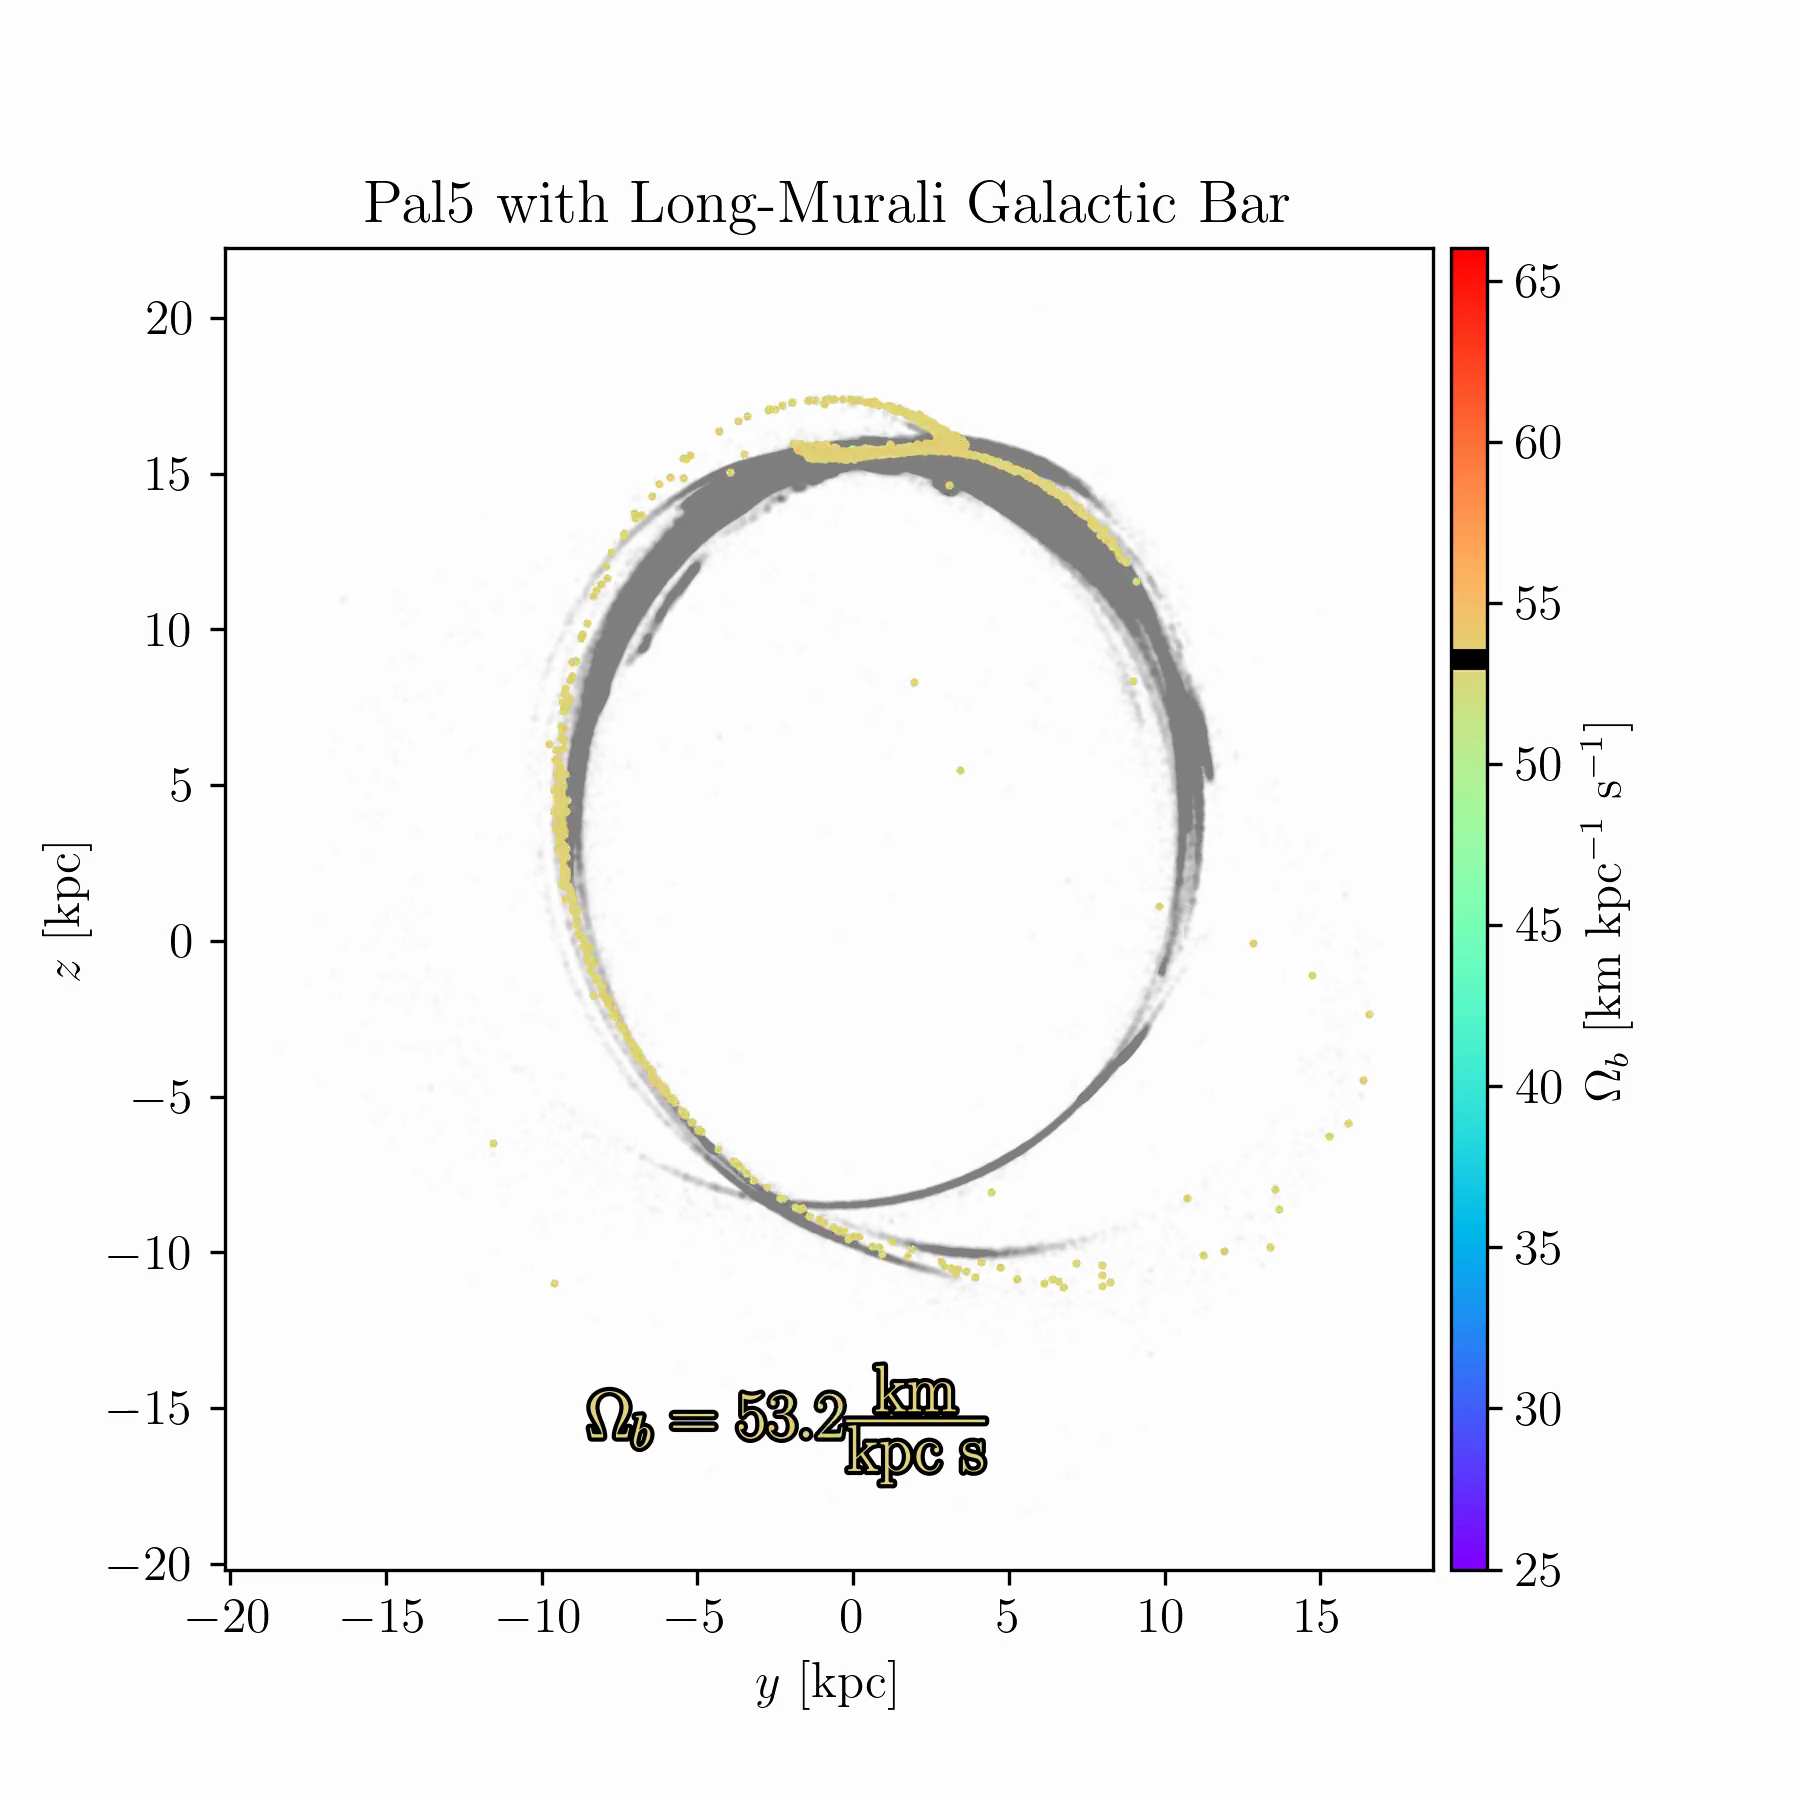
\includegraphics[width=.32\linewidth]{images/frame_0104.png}\\
                \end{tabular}
                \caption[The presence of a stellar bar with different rotational speeds damaging the Palomar~5 stream]{Various simulations of producing the Palomar~5 stream using \texttt{tstrippy} with 5000 particles. The galaxy was modeled using \citet{2017A&A...598A..66P} and the bar was modeled with \citet{1997MNRAS.291..717M}, as describe in chapter~4. However, we vary the bar pattern speed. We run the simulation for the same initial conditions but with the different bar pattern speeds. We varied the bar pattern speed between 25-61~km/(s~kpc) with a 150 samples. There is an animated version of this graph availble on the online version of this thesis.}
                \label{fig:pal5_with_bar}
            \end{figure}

    \subsection{Multiple-stellar populations, Stellar evolution, and globular cluster formation and internal dynamics, stellar populations}

        What if we wanted to go further? Indeed at somepoint, this is just considered other work or future considerations, or other research questions entirely. 

        What if we wanted to further? this is certainly outside the scope of our work, but we could consider the globular cluster formation. 

        The complexity doesn't end here. For instance, we are unsure how globular clusters form. There are some mechanisms proposed (cite the extra galactic GC review). That review summarizes them as: (1), (2), (3). However, to completely understand them would involve understanding the chemical enrichment history of the universe. Starting from big-bang nucleosysntehsis, to first generation stars (POP III), and how these first stars chemically enrich the environment, and how the clusters form from said environment. \citet{2022A&A...668A.191C} studied cluster formation in environments that were enriched by just pop II stars or a mixture of pop III/II stars and showed that pop III stars were necessary to enrich the environment enough to reproduce current cluster qualtities. 

        However, from my literature review there does seem to be a gap linking the chemical environment that could be enriched from a combination of pop II/popIII stars and how cluster formation. At least we know clusters are at least second generation (pop II) stars, since the first stars (pop III) form massive and die young \citep{2002ApJ...571...30S}.

        Ideally, we would like to know about the stars within the cluster to then infer the environment that it must have been born in. Extra-galactic census of globular clusters show that there isa bi-modality in color, making people believe that there are at least two generations or two different mechanisms for forming them. 

        \citet{2025arXiv250507491V} is looking at black hole formation inside of globular clusters that are being born. 

        \citet{2024A&A...681A..45L} Elena and Alessandra investigate a scenario that considers multiple populations in globular clusters where the second population is much less massive than the first, but evaporation and tidal stripping processes can mean that there present day contributions are similar to one another. 

        \citet{2025MNRAS.537.2342C} is looking at the dynamics of the different populations within 47 Tuc.

        \citet{2024MNRAS.529.2413U} said that there's evidence of multiple populations within the stellar streams. Something expected and now observationally confirmed     

        \citet{2025MNRAS.540.1235C} presents a cool scenario for investigating globular cluster formation during galaxy formation and mergers. They discuss the chemical environment the clusters form in as an enrichment process from POP III and POP II stars. I must read this more in detail. It is fascinating work. 

        \citet{2004AJ....127.2753D} presented a great work on Palomar~5 and found the parameters of a king model that best reproduce Palomar~5. Perhaps I can take form this study to have the best description of the tidal tails that corresponds to Palomar~5, and iterate over this to have the best description of of the tails as possible. 

        \citet{2006ARA&A..44..193B} made a review on extra galactic globular clusters. They discuss things like the observation evidence, the globular cluster mass function (all clusters), and find it to have an equal power spectrum, but the issue is that you don't know where to truncate the power law. maybe at lower end you can argue $10^4 M_\odot$ from two body relaxation and a tidal field. However, the upper limit is hard since you already don't expect that many, and the inclusion of a couple more high mass members can significantly alter the ``mean'' mass GC. They also note how a lot of cluster properties match the galactic properties. They talk about a bi-modal distribution. It really isn't that bimodal, there's a ton of overlap. There's a bluer one and a redder one. One of them might form during the collisions between galaxies while the other could be formed deeped in the potential wells. They also said that as of 2014 there is evidence that GCs are still forming. They also discuss the chemical abundance patterns within the clusters. It's complicated stuff, I wish I was better at stellar physics and knowing all the different sequences\dots

        Something about the chemical abundance patterns of the halo stars that can be consistent with the globular clusters \dots

        Schiavon (2017) showing that there exist many N-rich stars which have chemical abundance patterns similar to stars within the clusters all over the galactic field. 

        Fernández-Trincado, José G (2021) says that there are some metal rich cluster debris, which is interesting 

        Fernández-Trincado, J. G (2017) said they found 11 stars with the chemical abundance patterms of second general stars within globular cluster \dots 

\section{Future modeling techinques}

    I want to integrate these discussions in smoothly with the other scientific questions and not separate the modelling techinques. 

    \subsection{N-body codes}
    \citep{2012MNRAS.424..545N} showed the GPU's can replace GRAPE

    \citet{2018ComAC...5....2V} talks about a series of papers between a larger collaboration of people who specialize in collisional dynamics and who have performed a series of workshops together. The introduction stated that the collaboration wants to tackle many open questions regarding stellar clusters and build the necessary codes to interprete the future large quantity of data that was destined to come. It has now come since the review was 2018. An interesting point was that in general globular clusters are approximated as being orderless, i.e. isotropic but order does present itself within these stelalr systems. Another large problem is no one knows what a good set of initial conditiosn is. Unresolved binaries pose a problem because you can overestiamte the total mass of the system. If I talk about this review, I should probably discuss some of the results from the papers that is builds on or at least their techinques.

    The MODEST review led me to discover AMUSE, which is an framework for integrating various astrophysical codes for solving 4 types of problems: gravitational dynamics, radiative transfer, hydrodynamics, and stellar evolution. The codes are written by the community and are interfaced together with Amuse. The user end is python. I have spent some time reading the book, which is instructive and well written. Steve McMillian is one of the authors. The code has a large support on GitHub and is still being developped. I have had trouble trying to install the code. It seems as though their documentation is incoherrent. At one place, it said `pip' is the easiest way to install. It didn't work. In another place, I was instructed to install a zipped up tarball. The setup failed becuase it expected there to be a .git file in the directory. I successfully downloaded the code by cloneing the repository, despite the fact that this was not recommended. I can use some aspects of the code but not all of them. For instance, my memory tells me that about 80\% of the test suite passed, thus many scripts failed. This was when I only installed the frame-work, which was advised since installing the whole package is huge and unnecessary since I am not solving all astrophysical problems. However, I wasn't able to use one of the gravity solvers that was presented in the textbook `AstrophysicalRecipes The art of AMUSE'. The install still has some codes that failed for instance: amuse-adaptb, amuse-hermite-grx, amuse-mi6. However, I'm hoping that this isn't necessary. I want to educate myself and make some examples. 

    Installing other codes and figuring out their functionalities to me has never been trivial. This is similar to galpy when I tried to figure out particle spray method and got less than good results. Agama also confused me a bit. The main point is that for each package, at the end of the day I decided that it was easier and better if I solved the problem myself with my own code. Because, even with the other packages, I know that they can be used to solve other astrophysical problems and it wasn't clear to me how to make the codes solve my specific set of of the restricted three body problems in a potential with other perturbers flying around. 

    In this search, I also discovered another review called \textit{Computational methods for collisional stellar systems} by Spurzem and Kamlah 2023. It is also interesting and instructive. I found it insightful when they called NBody an industry. I think the story of GRAPE and Makino is really interesting, how he build dedicated hardware for the nbody problem which were great for 10 years but were quickly replaced by GPU technology. 







